                % Post-Quantum OIDC with KEMTLS -- LaTeX Report
                % Build (from repo root):
                %   python3 report/generate_assets.py
                %   cd report && pdflatex -interaction=nonstopmode main.tex && pdflatex -interaction=nonstopmode main.tex
                %
                % Notes:
                % - All benchmark numbers shown are derived from benchmark_results/benchmark_results.{csv,json}.
                % - This report avoids claims not supported by the checked-in code and artifacts.
                
                \documentclass[conference]{IEEEtran}
                
                % IEEE-style packages (keep this fairly minimal for portability on Overleaf).
                \usepackage[T1]{fontenc}
                \usepackage{graphicx}
                \usepackage{booktabs}
                \usepackage{longtable}
                \usepackage{array}
                \usepackage[table]{xcolor}
                \usepackage{listings}
                \usepackage{float}
                \usepackage{needspace}
                \usepackage{tikz}
                \usetikzlibrary{positioning,arrows.meta,fit,calc,backgrounds}
                \usepackage{placeins}
                \usepackage{url}
                \usepackage{hyperref}
                
                \hypersetup{
                  colorlinks=true,
                  linkcolor=blue!60!black,
                  urlcolor=blue!60!black,
                  citecolor=blue!60!black
                }
                
                % Reduce excessive vertical whitespace around floats/sections in IEEE two-column layout.
                \setlength{\textfloatsep}{8pt plus 2pt minus 2pt}
                \setlength{\floatsep}{6pt plus 2pt minus 2pt}
                \setlength{\intextsep}{8pt plus 2pt minus 2pt}
                \setlength{\abovecaptionskip}{3pt}
                \setlength{\belowcaptionskip}{3pt}
                
                % Breakable, monospaced file paths (prevents right-margin clipping with \texttt{...}).
                % Uses \path from hyperref/url but forces \ttfamily locally.
                \newcommand{\codepath}[1]{\begingroup\def\UrlFont{\ttfamily}\path{#1}\endgroup}
                
                \definecolor{codebg}{RGB}{248,248,248}
                \definecolor{layerA}{RGB}{230,245,255}
                \definecolor{layerB}{RGB}{229,245,224}
                \definecolor{layerC}{RGB}{255,244,229}
                \definecolor{layerD}{RGB}{245,229,255}
                
                \lstset{
                  basicstyle=\ttfamily\small,
                  backgroundcolor=\color{codebg},
                  frame=single,
                  rulecolor=\color{black!15},
                  aboveskip=0.6em,
                  belowskip=0.8em,
                  breaklines=true,
                  columns=fullflexible,
                  keepspaces=true
                }
                
                \title{Post-Quantum OpenID Connect with KEMTLS-Inspired Key Establishment: Prototype and Evaluation}
                \author{\IEEEauthorblockN{Aniket Gupta (IIT2023018)}
                \IEEEauthorblockA{Indian Institute of Information Technology, Allahabad\\Repository: \url{https://github.com/42-answer/PQC}}}
                
                \begin{document}
                \maketitle
                
                \begin{abstract}
                As quantum computing compromises classical cryptographic primitives, securing authentication infrastructure has become a critical objective. Standard Post-Quantum TLS (PQTLS) introduces severe performance overhead due to the massive size of post-quantum digital signatures. To address this, the presented Python prototype implements a KEMTLS-inspired key-establishment protocol, completely substituting digital signatures with highly efficient Key Encapsulation Mechanisms (KEMs) for both confidentiality and authentication. An OpenID Connect (OIDC) authorization pipeline is deployed over this transport layer, facilitating the issuance and verification of post-quantum signed JSON Web Tokens (PQ-JWTs). The end-to-end flow is accessible via a web interface and JSON APIs.

                Performance characteristics of the post-quantum primitives are evaluated using an integrated microbenchmarking suite. The reported quantitative metrics reflect in-process execution times and cryptographic payload sizes, ensuring deterministic reproducibility. The underlying system architecture is mapped, deviations from standard compliance are identified, and a roadmap toward production-ready network integration is outlined.
                \end{abstract}
                
                \begin{IEEEkeywords}
                post-quantum cryptography, Kyber (ML-KEM), ML-DSA, Falcon, KEMTLS, OpenID Connect, JWT, benchmarking.
                \end{IEEEkeywords}
                
                \section{Scope and Reproducibility}
                \subsection{Introduction}
                The transition to post-quantum cryptography is an urgent requirement for securing modern authentication systems against future quantum threats. The standard TLS 1.3 protocol achieves key establishment via ephemeral Diffie-Hellman and relies on digital signatures for server authentication. A straightforward approach to post-quantum security is Post-Quantum TLS (PQTLS), which operates as a direct drop-in replacement, substituting classical algorithms with post-quantum equivalents. However, post-quantum digital signatures (such as ML-DSA) present a significant drawback: their public keys and signatures are substantially larger than traditional algorithms like RSA or ECDSA. As illustrated in Figure~\ref{fig:kemtls_1}, PQTLS maintains the identical structural rounds and message flow of TLS 1.3 but inherits severe communication and computational overhead due to the massive size of these post-quantum signatures~\cite{celi2021kemtls}.

                To mitigate this overhead, we adopt an alternative protocol design called KEMTLS~\cite{kemtls, celi2021kemtls}. Because post-quantum Key Encapsulation Mechanisms (KEMs) are fundamentally more efficient and require smaller cryptographic material than post-quantum signatures, KEMTLS eliminates handshake signatures entirely. Instead, it leverages KEMs for both confidentiality and authentication. As depicted in Figure~\ref{fig:kemtls_2}, KEMTLS restructures the handshake flow: authentication is achieved by encapsulating a shared secret against the server's long-term post-quantum KEM public key, which is advertised in its certificate. Only the legitimate server possessing the corresponding private key can decapsulate this secret, authenticating the connection while circumventing the bandwidth penalties of post-quantum digital signatures.
                
                \begin{figure}[!t]
                \centering
                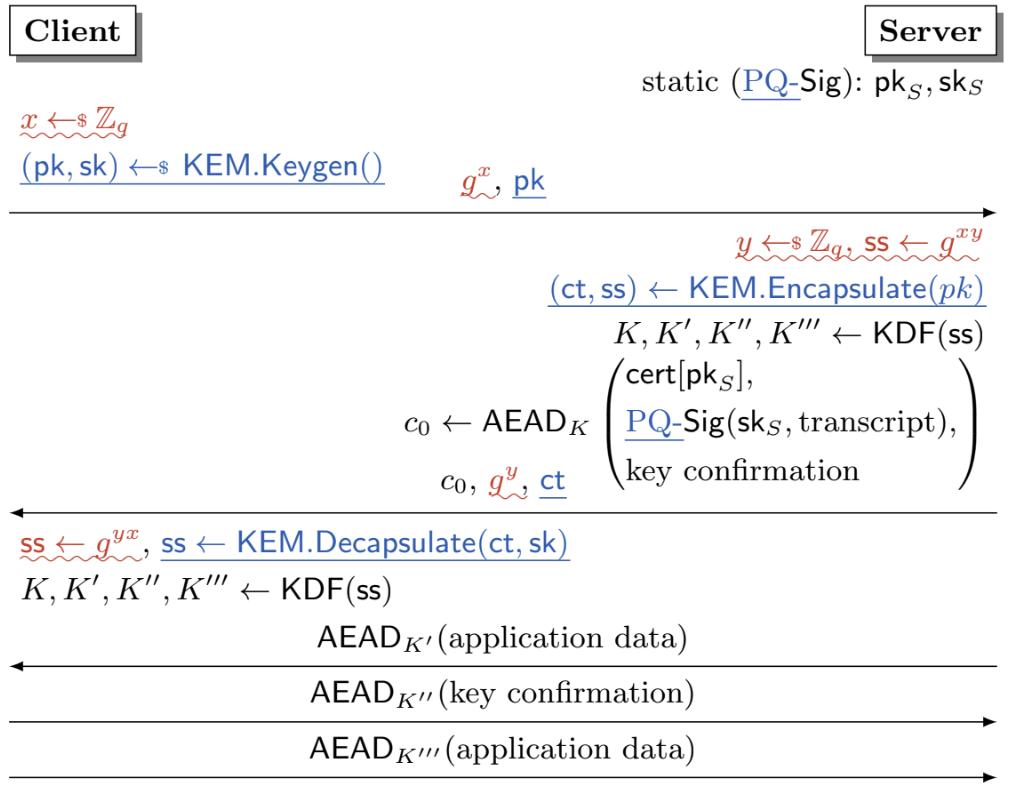
\includegraphics[width=\columnwidth]{figures/fig1.png}
                \caption{Comparison between TLS 1.3 handshake (black and red) and PQTLS (black and blue). Note that both protocols require the same number of rounds and messages~\cite{celi2021kemtls}.}
                \label{fig:kemtls_1}
                \end{figure}
                
                \begin{figure}[!t]
                \centering
                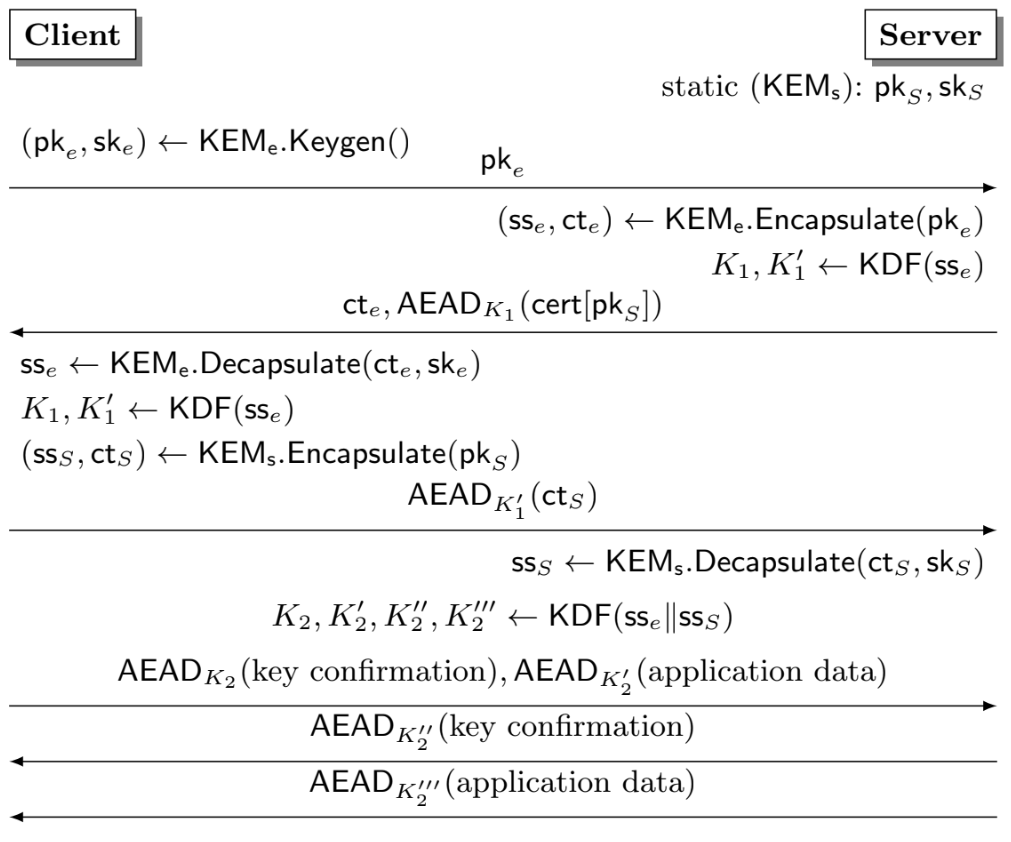
\includegraphics[width=\columnwidth]{figures/fig2.png}
                \caption{Overview of KEMTLS with server-only authentication~\cite{celi2021kemtls}.}
                \label{fig:kemtls_2}
                \end{figure}

                This optimized transport foundation supports an application-layer OpenID Connect (OIDC) authorization-code flow~\cite{rfc6749,oidc-core, li2015analysing}. The architecture is validated through an integrated microbenchmarking suite and a web-based interface. All quantitative results analyzed in this report are extracted directly from the generated artifacts to guarantee deterministic reproducibility.
                
                \noindent The primary technical contributions include:
                \begin{itemize}
                  \item \textbf{KEMTLS validation:} An implementation demonstrating the mitigation of post-quantum signature overhead via KEM-based authentication.
                  \item \textbf{Primitive integration:} A post-quantum wrapper layer exposing Kyber KEM and signature operations for modular composition.
                  \item \textbf{OIDC pipeline:} An authorization demonstrator generating and verifying post-quantum signed ID tokens.
                  \item \textbf{Reproducible methodology:} An artifact-driven reporting structure that programmatically translates benchmarking data into academic visualizations.
                \end{itemize}
                \noindent Project repository: \url{https://github.com/42-answer/PQC}
                
                \noindent The quantitative analysis relies exclusively on checked-in benchmark datasets (CSV/JSON).
                
                \subsection{How to Run (README-aligned summary)}
                The README documents a full setup using liboqs plus a Python virtual environment (Python 3.8+; tested on Linux/macOS). At a high level:
                \begin{itemize}
                  \item Install liboqs and ensure the shared library is discoverable (e.g., via \texttt{LD\_LIBRARY\_PATH}).
                  \item Activate the project environment via \texttt{source setup\_env.sh}.
                  \item Run the UI demo with \texttt{python ui/app.py} and optionally validate endpoints with \texttt{python test\_ui\_endpoints.py}.
                \end{itemize}
                \subsection{Standards Context and Related Work}
                The prototype is framed using established standards and prior work, without proposing new protocol specifications. The identity flow follows the structure of the OAuth~2.0 authorization-code exchange~\cite{rfc6749} and references the OIDC Core profile~\cite{oidc-core}; tokens use JWT/JWS container formats~\cite{rfc7519,rfc7515}. For key establishment, the prototype adopts the central KEMTLS idea of removing handshake signatures~\cite{kemtls}. The underlying KEM and signature algorithms align with NIST standardization outcomes and references~\cite{fips203,fips204,nist-pqc}. The implementation uses Open Quantum Safe tooling (liboqs and its Python bindings) to access PQ algorithms in a reproducible software stack~\cite{liboqs}.
                
                \noindent See detailed instructions in the GitHub repository README: \url{https://github.com/42-answer/PQC}
                
                \subsection{Code Layout (as used by this report)}
                The README organizes the implementation into the following components. This report uses the top-level layout (\texttt{src/}, \texttt{ui/}, \texttt{docs/}, \texttt{examples/}, \texttt{benchmark\_results/}, \texttt{report/}). A nested \texttt{PQC/} directory also exists with a similar structure; this report references the top-level paths.
                \begin{itemize}
                  \item \codepath{src/pq_crypto/}: wrappers for PQ KEM and signature operations.
                  \item \codepath{src/kemtls/}: KEMTLS protocol structures and client/server modules.
                  \item \codepath{src/oidc/}: PQ-signed JWT handling and an in-memory OIDC server/client.
                  \item \codepath{src/benchmarks/run_benchmarks.py}: benchmark execution logic.
                  \item \codepath{src/benchmarks/generate_pdf_report.py}: benchmark-report generation used by the benchmarking subsystem.
                  \item \codepath{src/docs/generate_technical_doc.py}: technical documentation generator.
                  \item \codepath{benchmark_results/benchmark_results.csv} and \codepath{benchmark_results/benchmark_results.json}: stored benchmark results used in all tables/figures.
                  \item \codepath{ui/app.py}: Flask UI demo and API endpoints.
                  \item \codepath{ui/templates/}: HTML templates for the demo pages.
                  \item \codepath{test_ui_endpoints.py}: smoke tests against the running UI.
                  \item \codepath{setup_env.sh}: environment activation (venv + liboqs paths), as documented in the README.
                  \item \codepath{examples/}: example scripts for running demo flows.
                  \item \codepath{docs/}: architecture and quickstart documents.
                  \item \codepath{report/}: this LaTeX report plus the asset generator used to produce figures and tables.
                \end{itemize}

                \subsection{Software Stack and Execution Environment}
                The prototype is implemented in Python and is intended to run inside a virtual environment created by \codepath{setup\_env.sh}. The setup script configures \texttt{PYTHONPATH} for in-repository imports and extends \texttt{LD\_LIBRARY\_PATH} so the system liboqs shared library can be located at runtime. The Flask UI additionally sets \texttt{OQS\_INSTALL\_DIR=/usr/local} to prefer an existing liboqs installation.

                \noindent The primary technologies and libraries used for the implementation and evaluation are:
                \begin{itemize}
                  \item \textbf{Post-quantum primitives:} liboqs via \texttt{liboqs-python} (\texttt{oqs} module) for Kyber KEM and PQ signature algorithms~\cite{liboqs}.
                  \item \textbf{Web demonstration:} Flask (and Flask-CORS) for the UI and JSON API endpoints (\codepath{ui/app.py}).
                  \item \textbf{Benchmarking harness:} an in-process microbenchmark runner built around \texttt{time.perf\_counter()} (\codepath{src/benchmarks/run\_benchmarks.py}).
                  \item \textbf{Plotting and report assets:} NumPy and Matplotlib for generating figures and LaTeX table fragments from stored artifacts (\codepath{report/generate\_assets.py}).
                  \item \textbf{Endpoint validation:} the \texttt{requests} HTTP client for smoke-testing UI endpoints (\codepath{test\_ui\_endpoints.py}).
                  \item \textbf{Build toolchain:} \LaTeX{} (IEEEtran class, TikZ, and listings) for PDF generation from \codepath{report/main.tex}.
                \end{itemize}
                \noindent The repository also declares additional Python dependencies (e.g., PyJWT, Authlib, cryptography, python-dotenv, and PyYAML) that are common in OAuth/JWT ecosystems. In this prototype, the PQ-JWT handler implements JWT serialization explicitly to keep the token format and signature inputs easy to inspect.

                \subsection{Reproduction Pipeline}
                The following pipeline reproduces the report assets (tables/figures) from stored benchmark artifacts. It does not re-run cryptographic benchmarks; it re-plots and re-tabulates the existing results.
                
              \begin{lstlisting}[
language=bash,
caption={Re-creating figures and tables used by this report.},
captionpos=b
]
# from repo root
source setup_env.sh
python3 report/generate_assets.py
# build the PDF (pdflatex must be installed)
cd report
pdflatex -interaction=nonstopmode main.tex
pdflatex -interaction=nonstopmode main.tex
\end{lstlisting}


                \medskip
                
                \section{OpenID Connect Architecture}
                Securing the transport layer must be paired with robust application-layer identity workflows. OpenID Connect 1.0~\cite{oidc-core} establishes an identity layer atop the OAuth 2.0 framework~\cite{rfc6749}. While OAuth 2.0 governs profile authorization, OpenID Connect introduces definitive identity management, enabling a Relying Party (RP) to cryptographically verify user authenticity via an OpenID Provider (OP)~\cite{li2015analysing}.

                As outlined by Li and Mitchell~\cite{li2015analysing}, the OpenID Connect ecosystem relies on interactions between four core entities:
                \begin{enumerate}
                    \item \textbf{End User (U):} The person attempting to access protected resources.
                    \item \textbf{User Agent (UA):} Typically a web browser routing requests and responses.
                    \item \textbf{OpenID Provider (OP):} The server (e.g., Google or our Flask implementation) that authenticates the user and generates identity assertions.
                    \item \textbf{Relying Party (RP):} The application providing the online service, which consumes the OP's identity assertions to grant access.
                \end{enumerate}

                \begin{figure}[H]
                \centering
                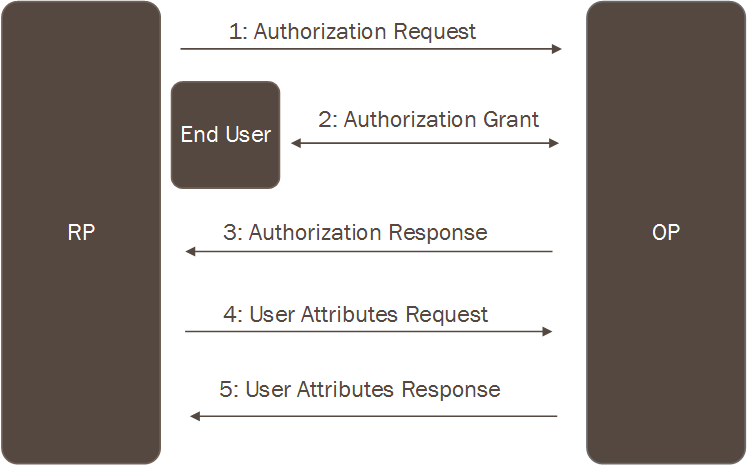
\includegraphics[width=\columnwidth]{figures/fig_oidc_1.png}
                \caption{Interactions within the OpenID Connect framework during authentication. Our prototype secures the generated identity tokens using post-quantum signatures~\cite{li2015analysing}.}
                \label{fig:oidc_1}
                \end{figure}
                
                The implemented prototype executes an OIDC authorization-code sequence where the OpenID Provider issues JSON Web Tokens (JWTs) as identity assertions. Standard RSA/ECDSA signing algorithms are substituted with post-quantum equivalents, producing PQ-signed JWTs that conform to the existing OpenID Connect specification.

                \section{System Architecture}
                \subsection{Layered Design}
                The architectural design is strictly layered: post-quantum primitives form the base, followed by a KEMTLS key-establishment protocol~\cite{kemtls}, and culminating in the OIDC application flow. Figure~\ref{fig:layered-arch} details this structural hierarchy in relation to the codebase modules.
                
                This stack operates in two modes. Functionally, the web interface triggers in-process endpoints executing the OAuth~2.0 and OIDC authorization sequence~\cite{rfc6749,oidc-core}. This mechanism handles the issuance and verification of ID tokens within standard JWT/JWS containers~\cite{rfc7519,rfc7515}. Analytically, the benchmark module evaluates primitive operations and end-to-end performance. The ``KEMTLS handshake'' metric specifically measures a simulated key establishment (encapsulation, decapsulation, and HKDF key derivation~\cite{rfc5869}), representing the cryptographic processing overhead independent of network latency~\cite{rfc8446}.
                
                \begin{figure*}[!t]
                \centering
                \begin{tikzpicture}[
                  box/.style={draw,rounded corners,thick,align=left,text width=0.90\linewidth,inner sep=10pt},
                  arr/.style={-Latex,very thick,shorten >=2pt,shorten <=2pt}
                ]
                \node[box,fill=layerA] (l4) {\textbf{Layer 4: OIDC-style application flow}\\\textit{Modules:} \codepath{src/oidc/server.py}, \codepath{src/oidc/client.py}, \codepath{ui/app.py}\\Authorization-code style flow: authenticate $\rightarrow$ authorization code $\rightarrow$ token exchange $\rightarrow$ ID token verification (OIDC Core~1.0 as reference~\cite{oidc-core}).};
                \node[box,fill=layerB,below=10pt of l4] (l3) {\textbf{Layer 3: Application security (PQ-signed JWT/JWS)}\\\textit{Module:} \codepath{src/oidc/pq_jwt.py}\\JWT creation/verification using ML-DSA (FIPS~204~\cite{fips204}) and Falcon (NIST PQC project~\cite{nist-pqc}) wrappers.};
                \node[box,fill=layerC,below=10pt of l3] (l2) {\textbf{Layer 2: KEMTLS-inspired key establishment}\\\textit{Modules:} \codepath{src/kemtls/}, \codepath{src/pq_crypto/utils.py}\\Kyber/ML-KEM key establishment (FIPS~203~\cite{fips203}); shared secret expanded using HKDF with SHA-256 (repository implementation).};
                \node[box,fill=layerD,below=10pt of l2] (l1) {\textbf{Layer 1: Post-quantum primitives and sizes}\\\textit{Modules:} \codepath{src/pq_crypto/kem.py}, \codepath{src/pq_crypto/signature.py}\\Kyber, ML-DSA, Falcon via liboqs/liboqs-python bindings~\cite{liboqs}.};
                
                \draw[arr] (l4.south) -- (l3.north);
                \draw[arr] (l3.south) -- (l2.north);
                \draw[arr] (l2.south) -- (l1.north);
                \end{tikzpicture}
                \caption{Layered architecture diagram aligned with the repository implementation.}
                \label{fig:layered-arch}
                \end{figure*}
                \subsection{Implementation Mapping to Repository Modules}
                To keep the architecture verifiable, we map each conceptual layer to the specific source files that implement it and note how those files are exercised. This mapping also makes the evaluation path explicit: the Flask UI drives the demo endpoints, the benchmark runner defines the timed regions and writes CSV/JSON artifacts, and the report pipeline consumes those artifacts to produce plots and tables.
                \noindent Primary implementation paths used by the demo and benchmark suite:
                \begin{itemize}
                  \item \textbf{Layer 1 (primitives):} \codepath{src/pq_crypto/kem.py}, \codepath{src/pq_crypto/signature.py}, \codepath{src/pq_crypto/utils.py}.
                  \item \textbf{Layer 2 (KEMTLS-style):} \codepath{src/kemtls/protocol.py} plus \codepath{src/kemtls/client.py} and \codepath{src/kemtls/server.py}.
                  \item \textbf{Layer 3 (PQ-JWT):} \codepath{src/oidc/pq_jwt.py}.
                  \item \textbf{Layer 4 (OIDC-style demo):} \codepath{src/oidc/server.py}, \codepath{src/oidc/client.py}, and the UI wiring in \codepath{ui/app.py}.
                  \item \textbf{Benchmarks and artifacts:} \codepath{src/benchmarks/run_benchmarks.py}, stored results under \codepath{benchmark_results/}, and report-asset generation via \codepath{report/generate_assets.py}.
                \end{itemize}
                \noindent Implementation-level interaction (how the layers compose in code):
                \begin{itemize}
                  \item \textbf{Primitive wrappers and KDF utilities.} The PQ wrappers in \codepath{src/pq_crypto/} provide a thin integration layer over liboqs (via \texttt{liboqs-python}) for KEM and signature operations. The same package also contains utility code (e.g., HKDF-style expansion using SHA-256 in repository code) that is reused by higher layers.
                  \item \textbf{KEMTLS-inspired key establishment.} The modules under \codepath{src/kemtls/} define message structures and client/server roles suitable for a KEMTLS-inspired handshake. For evaluation, the stored ``Full KEMTLS Handshake'' row corresponds to a benchmark-suite simulation built from the same underlying KEM operations and key derivation logic, executed in-process.
                  \item \textbf{PQ-signed JWT handling.} The token logic in \codepath{src/oidc/pq_jwt.py} constructs and verifies JWT/JWS-style containers while delegating signing and verification to the PQ signature wrappers.
                  \item \textbf{OIDC-style flow orchestration.} The in-memory OIDC server/client modules under \codepath{src/oidc/} implement the authorization-code style sequencing used by the demo (authorization, code issuance, token exchange, ID token verification). The Flask UI endpoints in \codepath{ui/app.py} call into these modules to execute the flow as a single in-process sequence.
                \end{itemize}
                \noindent Methodology hook (where measurements attach): the benchmark runner in \codepath{src/benchmarks/run_benchmarks.py} defines the measurement boundaries for each artifact row. Primitive-level rows wrap individual operations (key generation, encapsulation/decapsulation, signing/verification). Protocol-level rows wrap complete in-process sequences: the KEMTLS-style key-establishment simulation and the end-to-end OIDC-style flow. These timings are written to CSV/JSON under \codepath{benchmark_results/} and are subsequently transformed into figures and tables by \codepath{report/generate_assets.py}.
                
                \subsection{Implementation Status and Coverage}
                The repository contains both core implementations and prototype wiring:
                \begin{itemize}
                  \item \textbf{Implemented primitives:} Kyber KEM operations and PQ signatures (ML-DSA variants, Falcon variants) are wrapped and benchmarked.
                  \item \textbf{KEMTLS components:} protocol structures and client/server modules exist; the benchmarked ``Full KEMTLS Handshake'' in stored results corresponds to a key-establishment simulation implemented in the benchmark suite (KEM encaps/decaps + key derivation).
                  \item \textbf{OIDC demo flow:} the Flask UI endpoint \texttt{/api/oidc/flow} executes an in-process authorization-code style sequence via server methods and PQ-signed ID token verification. The final ``UserInfo'' step is simplified to a direct user lookup (not a full bearer-token validated UserInfo implementation).
                \end{itemize}
                \subsection{Implementation-Centric Architecture Views}
                Beyond the conceptual layering, Figures~\ref{fig:module-arch} and~\ref{fig:endtoend-arch} illustrate how the repository modules connect in practice.
                
                \begin{figure*}[!t]
                \centering
                \begin{tikzpicture}[
                  font=\small,
                  m/.style={draw,rounded corners,thick,align=center,inner sep=6pt,text width=3.10cm},
                  arr/.style={-Latex,very thick,shorten >=4pt,shorten <=4pt},
                  grp/.style={draw,rounded corners,thick,inner sep=8pt,fill=black!2}
                ]
                
                % Top row: runtime call/dependency chain (left -> right).
                \node[m,fill=layerA] (ui) {\codepath{ui/app.py}\\Flask demo UI/APIs};
                \node[m,fill=layerB,right=12pt of ui] (oidc) {\codepath{src/oidc/}\\PQ-JWT + server/client};
                \node[m,fill=layerC,right=12pt of oidc] (kemtls) {\codepath{src/kemtls/}\\protocol + client/server};
                \node[m,fill=layerD,right=12pt of kemtls] (pq) {\codepath{src/pq_crypto/}\\KEM + signatures + HKDF};
                
                % Bottom row: benchmarks and stored artifacts.
                \node[m,fill=black!8,below=14pt of kemtls] (bench) {\codepath{src/benchmarks/}\\microbench suite};
                \node[m,fill=black!8,below=12pt of bench] (art) {\codepath{benchmark_results/}\\CSV + JSON};
                
                % Runtime dependencies.
                \draw[arr] (ui.east) -- (oidc.west);
                \draw[arr] (oidc.east) -- (kemtls.west);
                \draw[arr] (kemtls.east) -- (pq.west);
                
                % Modules pointing to benchmark suite
                \draw[arr] (kemtls.south) -- (bench.north);
                \draw[arr] (oidc.south) -- (bench.north west);
                \draw[arr] (pq.south) -- (bench.north east);
                
                % Benchmark writes artifacts
                \draw[arr] (bench.south) -- (art.north);
                
                % UI reads stored artifacts
                \draw[arr] (ui.south) to[out=-90,in=180] (art.west);
                
                % Grouping box behind nodes
                \begin{scope}[on background layer]
                \node[grp,fit=(pq) (kemtls) (oidc) (ui) (bench) (art)] {};
                \end{scope}
                
                \end{tikzpicture}
                \caption{Module-level architecture (arrows denote calls/reads in the repository; the benchmark suite writes stored artifacts).}
                \label{fig:module-arch}
                \end{figure*}
                
                \begin{figure*}[!t]
                \centering
                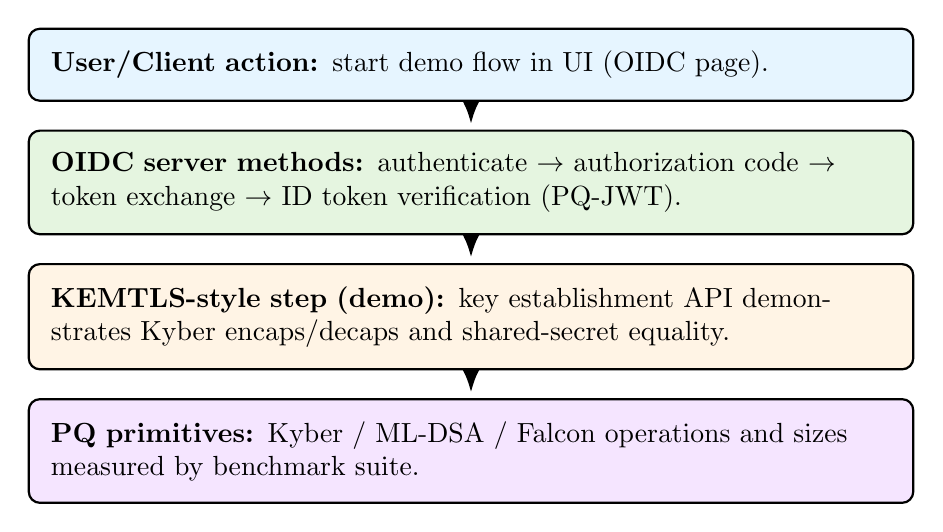
\begin{tikzpicture}[
                  s/.style={draw,rounded corners,thick,align=left,inner sep=8pt,text width=0.88\linewidth},
                  arr/.style={-Latex,very thick,shorten >=2pt,shorten <=2pt}
                ]
                \node[s,fill=layerA] (step1) {\textbf{User/Client action:} start demo flow in UI (OIDC page).};
                \node[s,fill=layerB,below=10pt of step1] (step2) {\textbf{OIDC server methods:} authenticate $\rightarrow$ authorization code $\rightarrow$ token exchange $\rightarrow$ ID token verification (PQ-JWT).};
                \node[s,fill=layerC,below=10pt of step2] (step3) {\textbf{KEMTLS-style step (demo):} key establishment API demonstrates Kyber encaps/decaps and shared-secret equality.};
                \node[s,fill=layerD,below=10pt of step3] (step4) {\textbf{PQ primitives:} Kyber / ML-DSA / Falcon operations and sizes measured by benchmark suite.};
                
                \draw[arr] (step1.south) -- (step2.north);
                \draw[arr] (step2.south) -- (step3.north);
                \draw[arr] (step3.south) -- (step4.north);
                \end{tikzpicture}
                \caption{End-to-end architecture view of the prototype pipeline (implementation-aligned).}
                \label{fig:endtoend-arch}
                \end{figure*}
                
                \section{Demo and Evaluation Pipelines}
                \subsection{Flask Demo UI Pipeline}
                The UI exposes routes for demonstrations and JSON APIs. The smoke-test script \texttt{test\_ui\_endpoints.py} checks that the following APIs return structured results when the UI is running:
                \begin{itemize}
                  \item \texttt{POST /api/kemtls/handshake}: Kyber keygen + encaps + decaps and shared-secret equality check.
                  \item \texttt{POST /api/signatures/test}: keygen + sign + verify; includes a negative test.
                  \item \texttt{POST /api/jwt/create}: create and verify a PQ-signed JWT; returns token size.
                  \item \texttt{POST /api/oidc/flow}: runs a five-step demo flow (authentication, code generation, token exchange, ID token verification, simplified userinfo retrieval).
                \end{itemize}
                
                \noindent Separately, the UI also exposes \texttt{GET /api/benchmarks} to return the stored benchmark JSON used for visualization (this endpoint is used by the UI pages but is not exercised by \texttt{test\_ui\_endpoints.py}).
                
                \Needspace{10\baselineskip}
                \subsection{UI Pipeline Diagram}
                The project includes a lightweight Flask-based UI that provides interactive pages and JSON API endpoints for demonstrating the prototype's post-quantum components. The UI supports a KEMTLS-style handshake demonstration (Kyber encaps/decaps and shared-secret check), PQ signature testing, PQ-signed JWT creation/verification, and an OIDC-style authorization-code flow.

                The following diagram is a compact, implementation-aligned view of how the UI is executed and validated.
                \Needspace{14\baselineskip}
                \begin{figure}[H]
                \centering
                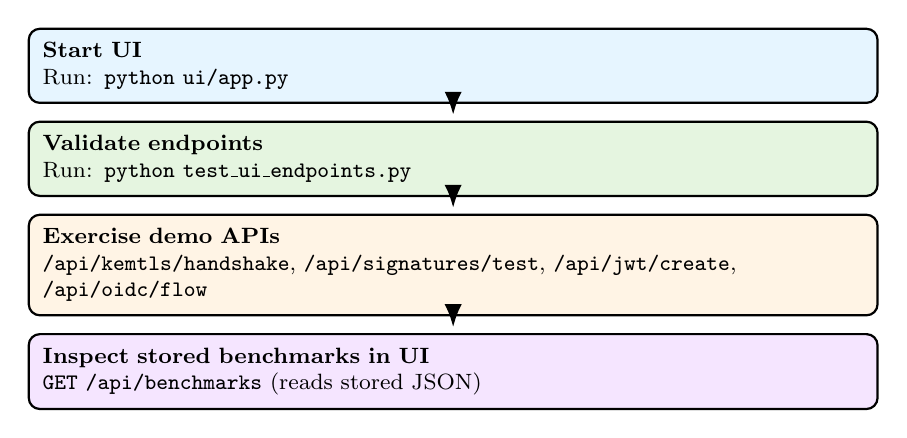
\begin{tikzpicture}[
                  font=\footnotesize,
                  p/.style={draw,rounded corners,thick,align=left,inner sep=5pt,text width=0.86\linewidth},
                  arr/.style={-Latex,very thick,shorten >=2pt,shorten <=2pt}
                ]
                \node[p,fill=layerA] (p1) {\textbf{Start UI}\\Run: \texttt{python ui/app.py}};
                \node[p,fill=layerB,below=6pt of p1] (p2) {\textbf{Validate endpoints}\\Run: \texttt{python test\_ui\_endpoints.py}};
                \node[p,fill=layerC,below=6pt of p2] (p3) {\textbf{Exercise demo APIs}\\
                \texttt{/api/kemtls/handshake}, \texttt{/api/signatures/test}, \texttt{/api/jwt/create}, \texttt{/api/oidc/flow}};
                \node[p,fill=layerD,below=6pt of p3] (p4) {\textbf{Inspect stored benchmarks in UI}\\
                \texttt{GET /api/benchmarks} (reads stored JSON)};
                
                \draw[arr] (p1.south) -- (p2.north);
                \draw[arr] (p2.south) -- (p3.north);
                \draw[arr] (p3.south) -- (p4.north);
                \end{tikzpicture}
                \caption{UI pipeline with implementation-aligned steps.}
                \label{fig:ui-pipeline}
                \end{figure}
                
                \Needspace{10\baselineskip}
                \subsection{Benchmark \texorpdfstring{$\rightarrow$}{->} Report Pipeline}
                This diagram summarizes how benchmark execution produces stored artifacts, which are then transformed into report-ready figures and tables.
                \begin{figure}[!t]
                \centering
                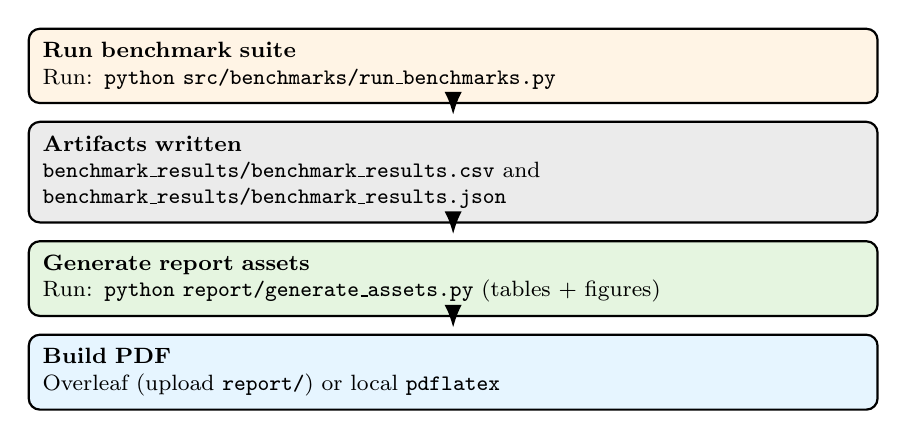
\begin{tikzpicture}[
                  font=\footnotesize,
                  p/.style={draw,rounded corners,thick,align=left,inner sep=5pt,text width=0.86\linewidth},
                  arr/.style={-Latex,very thick,shorten >=2pt,shorten <=2pt}
                ]
                \node[p,fill=layerC] (b1) {\textbf{Run benchmark suite}\\Run: \texttt{python src/benchmarks/run\_benchmarks.py}};
                \node[p,fill=black!8,below=6pt of b1] (b2) {\textbf{Artifacts written}\\\texttt{benchmark\_results/benchmark\_results.csv} and \texttt{benchmark\_results/benchmark\_results.json}};
                \node[p,fill=layerB,below=6pt of b2] (b3) {\textbf{Generate report assets}\\Run: \texttt{python report/generate\_assets.py} (tables + figures)};
                \node[p,fill=layerA,below=6pt of b3] (b4) {\textbf{Build PDF}\\Overleaf (upload \texttt{report/}) or local \texttt{pdflatex}};
                
                \draw[arr] (b1.south) -- (b2.north);
                \draw[arr] (b2.south) -- (b3.north);
                \draw[arr] (b3.south) -- (b4.north);
                \end{tikzpicture}
                \caption{Benchmark-to-report pipeline from execution to PDF generation.}
                \label{fig:bench-report-pipeline}
                \end{figure}
                
                \subsection{Benchmarking Pipeline}
                The benchmark suite in \codepath{src/benchmarks/run_benchmarks.py} measures:
                \begin{enumerate}
                  \item Kyber KEM keygen/encapsulation/decapsulation (three Kyber variants),
                  \item PQ signature keygen/sign/verify (ML-DSA and Falcon variants),
                  \item JWT creation and verification (subset of signature algorithms),
                  \item a ``Full KEMTLS Handshake'' simulation (key establishment + HKDF-based derivation),
                  \item an ``End-to-End OIDC Flow'' benchmark (in-process demo sequence).
                \end{enumerate}
                
                The stored results contain 32 benchmark rows (see Appendix~\ref{app:full-table}).
                
                \section{Benchmarking and Results (Stored Artifacts)}
                \subsection{Dataset and Provenance}
                All benchmark figures and tables in Section~4 are derived from the checked-in artifacts: \codepath{benchmark_results/benchmark_results.csv} and \codepath{benchmark_results/benchmark_results.json}. The plotting and tabulation script \codepath{report/generate_assets.py} is data-driven and produces the included PNG plots and LaTeX table fragments.
                
                \subsection{Metrics Summary (from stored artifacts)}
                The stored dataset contains \textbf{32} benchmark rows spanning \textbf{10} distinct operations and \textbf{10} configurations/algorithm labels.
                Key dataset-level metrics (microbenchmarks, in-process):
                \begin{itemize}
                  \item \textbf{Protocol-level timings (mean ms):} Full KEMTLS Handshake \(\approx 0.0409\) ms; End-to-End OIDC Flow \(\approx 0.2049\) ms.
                  \item \textbf{Kyber KEM operation means (ms):} observed range across Kyber512/768/1024 keygen/encap/decap is approximately \(0.0129\) to \(0.1003\) ms in the stored artifacts.
                  \item \textbf{JWT sizes (bytes):} ID token sizes produced by \emph{JWT Creation} range from \textbf{1193} to \textbf{4734} bytes across the benchmarked algorithms (verification rows record size as 0 in the artifacts).
                  \item \textbf{Signature sizes (bytes):} signature sizes recorded for signing range from \textbf{656} to \textbf{4627} bytes in the stored artifacts.
                \end{itemize}
                \subsection{KEM Operation Timings (Kyber)}
                This subsection summarizes key generation, encapsulation, and decapsulation timings across Kyber variants in the stored dataset.
                \begin{figure}[H]
                \centering
                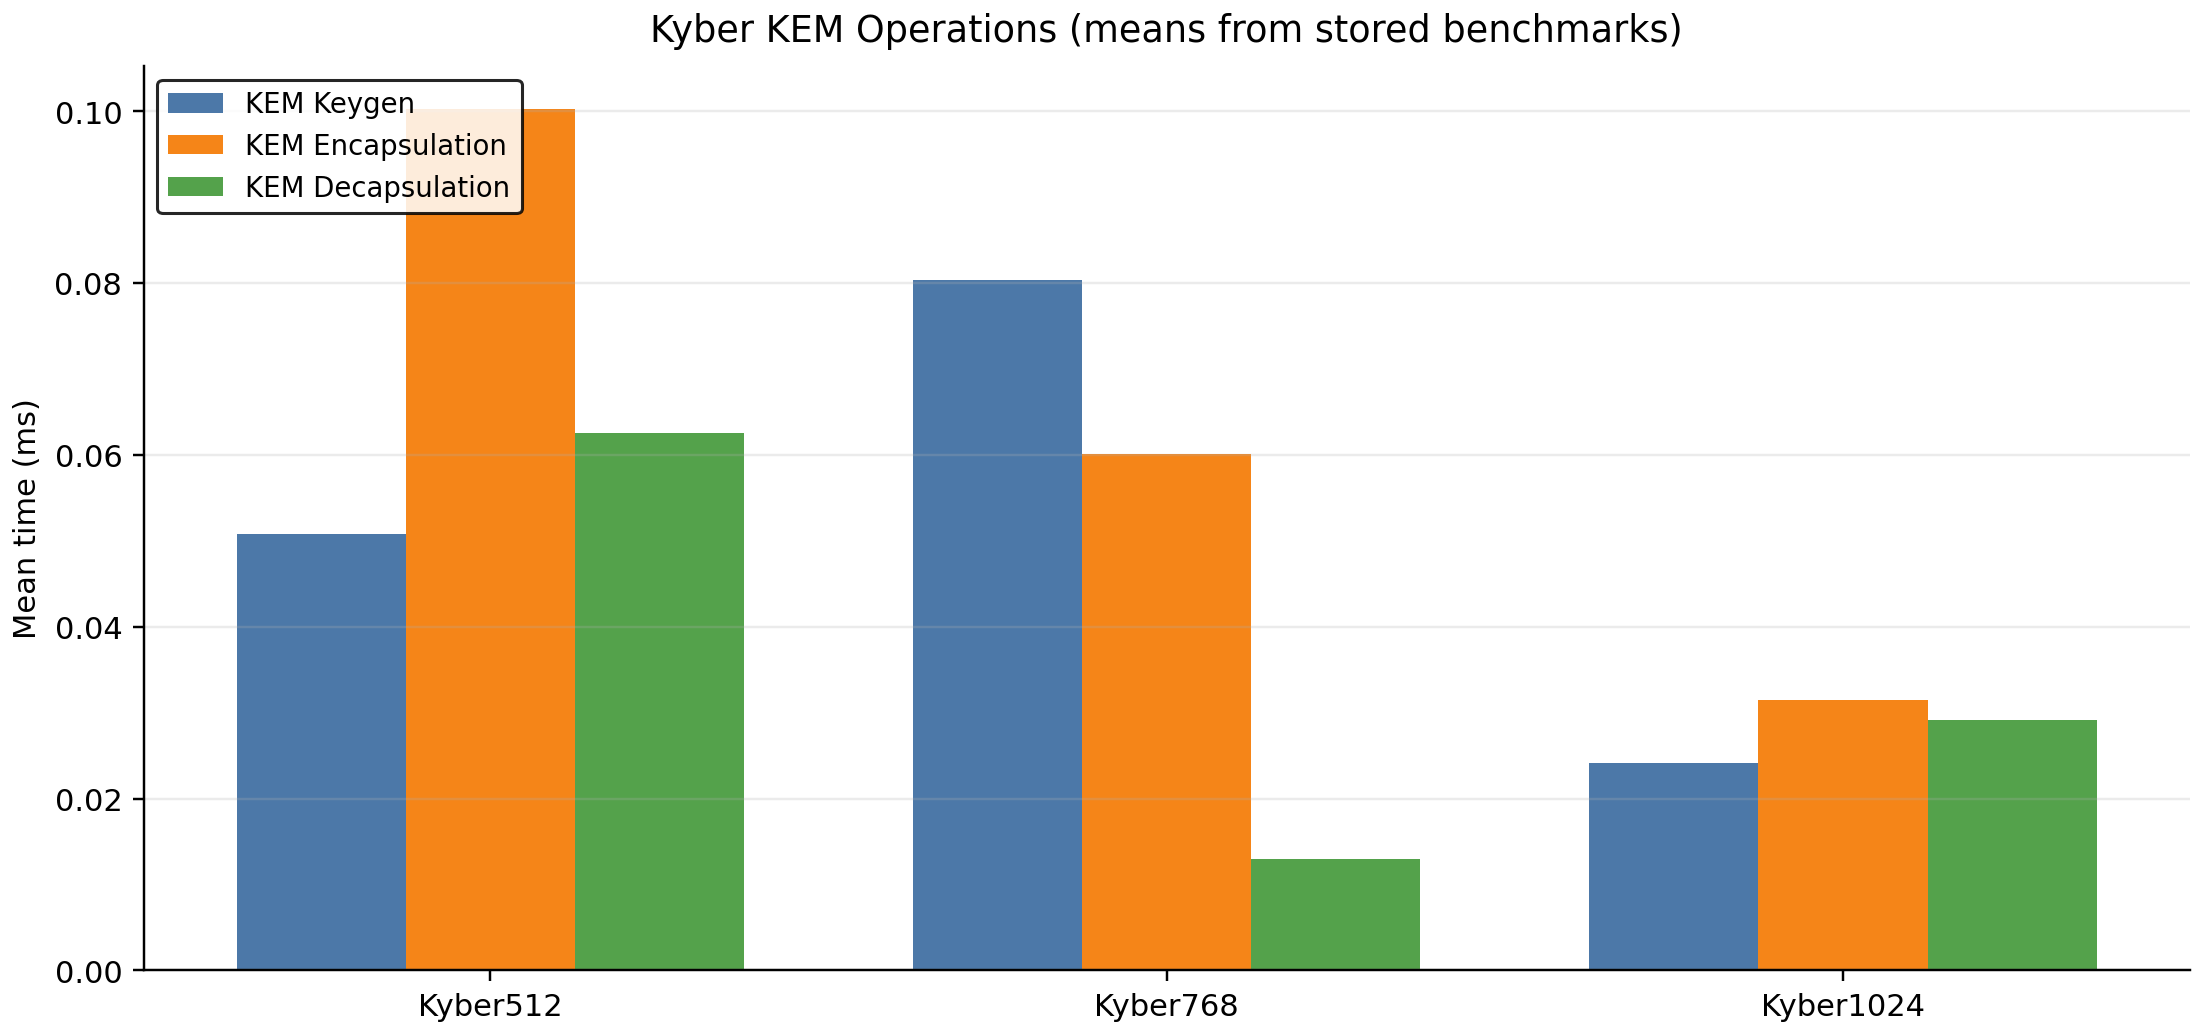
\includegraphics[width=\columnwidth]{figures/fig_kem_ops.png}
                \caption{Kyber KEM operation means (ms) from stored results.}
                \label{fig:kem-ops}
                \end{figure}
                \subsection{Signature Timings (ML-DSA and Falcon)}
                This subsection reports signing and verification timings across ML-DSA and Falcon variants as benchmarked in-process.
                \begin{figure}[H]
                \centering
                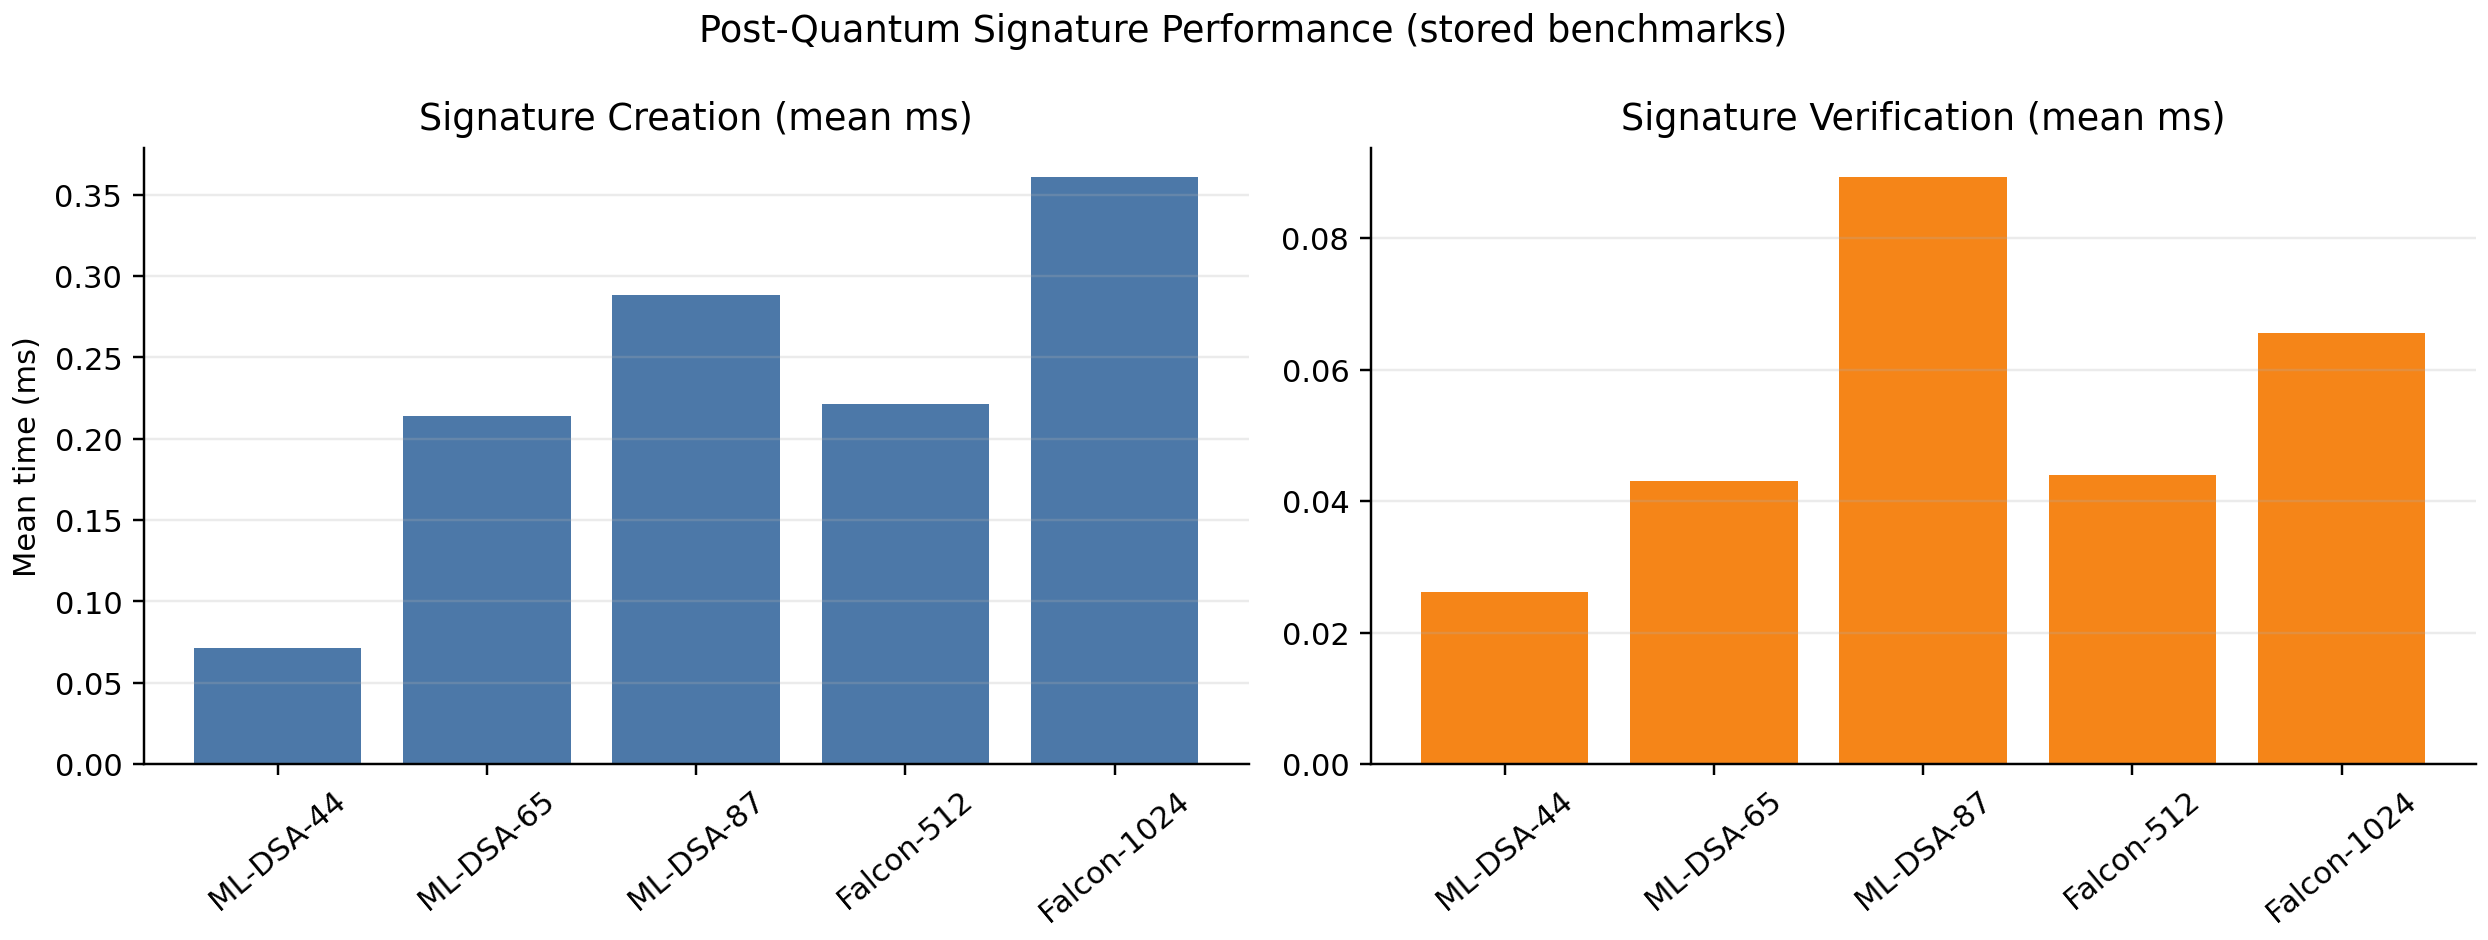
\includegraphics[width=\columnwidth]{figures/fig_signature_ops.png}
                \caption{Signature creation and verification means (ms) from stored results.}
                \label{fig:sig-ops}
                \end{figure}
                \subsection{JWT Performance and Token Sizes}
                This subsection reports JWT creation/verification time and the resulting ID token sizes for the PQ-signed JWT implementation.
                \begin{figure}[H]
                \centering
                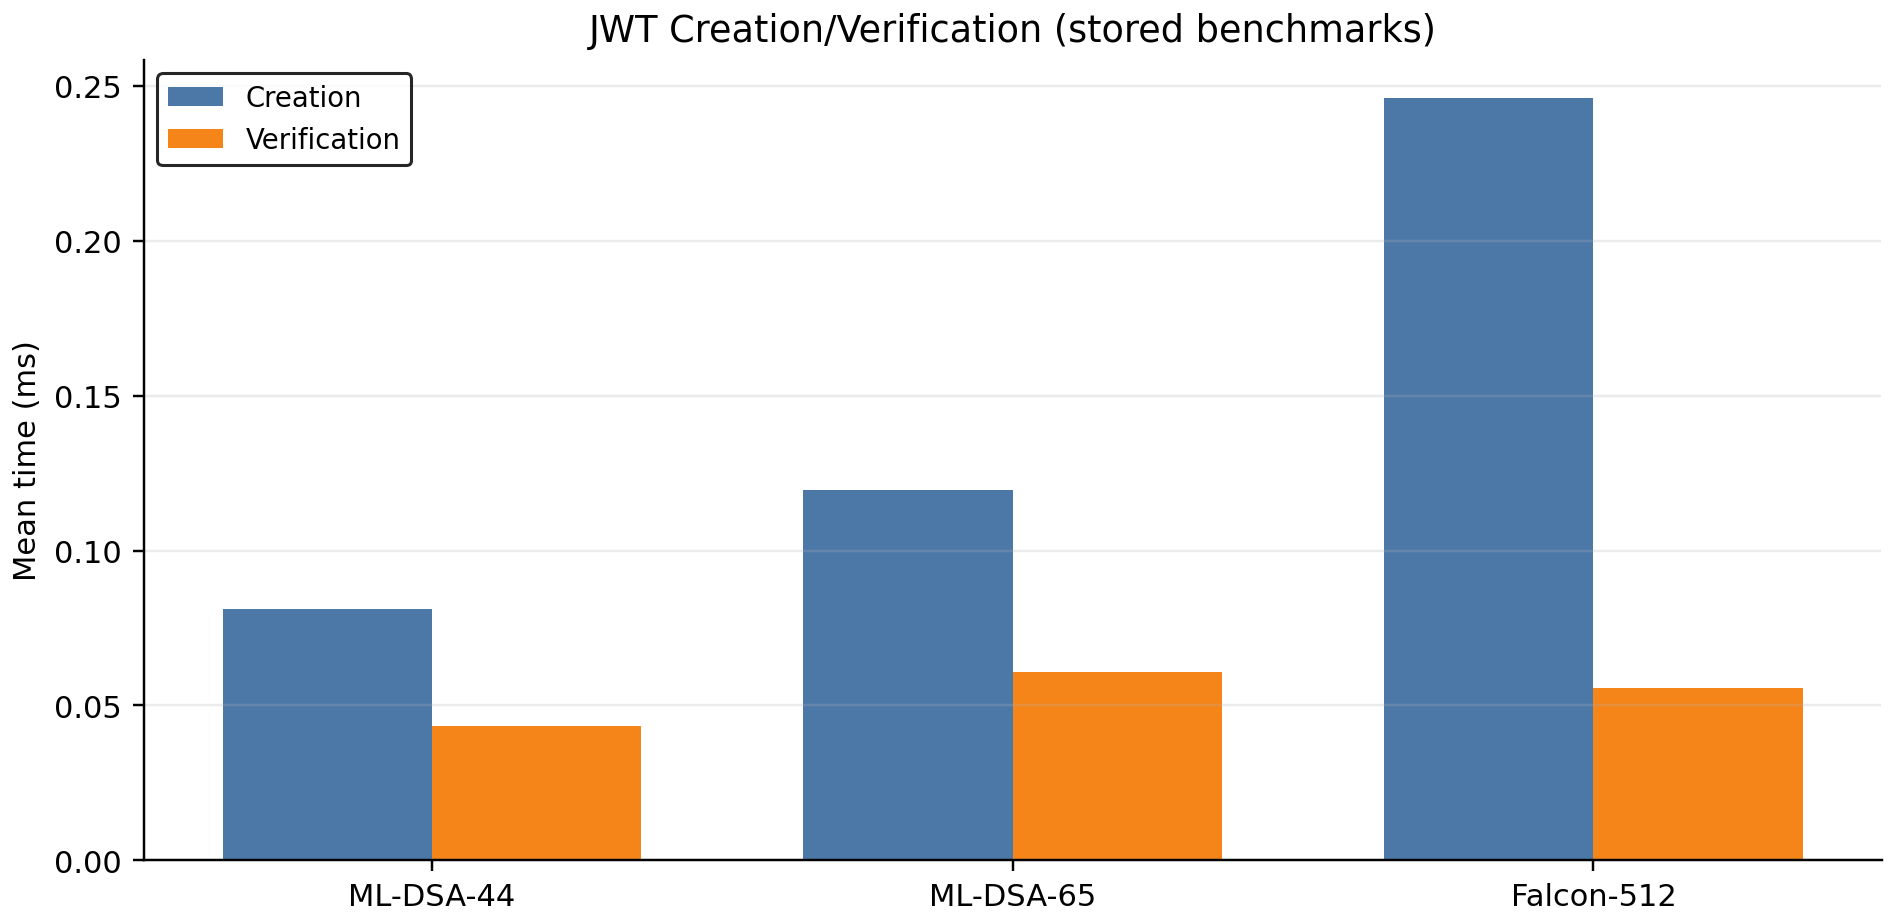
\includegraphics[width=\columnwidth]{figures/fig_jwt_ops.png}
                \caption{JWT creation vs. verification time (means, stored benchmarks).}
                \label{fig:jwt-times}
                \end{figure}
                
                \begin{figure}[H]
                \centering
                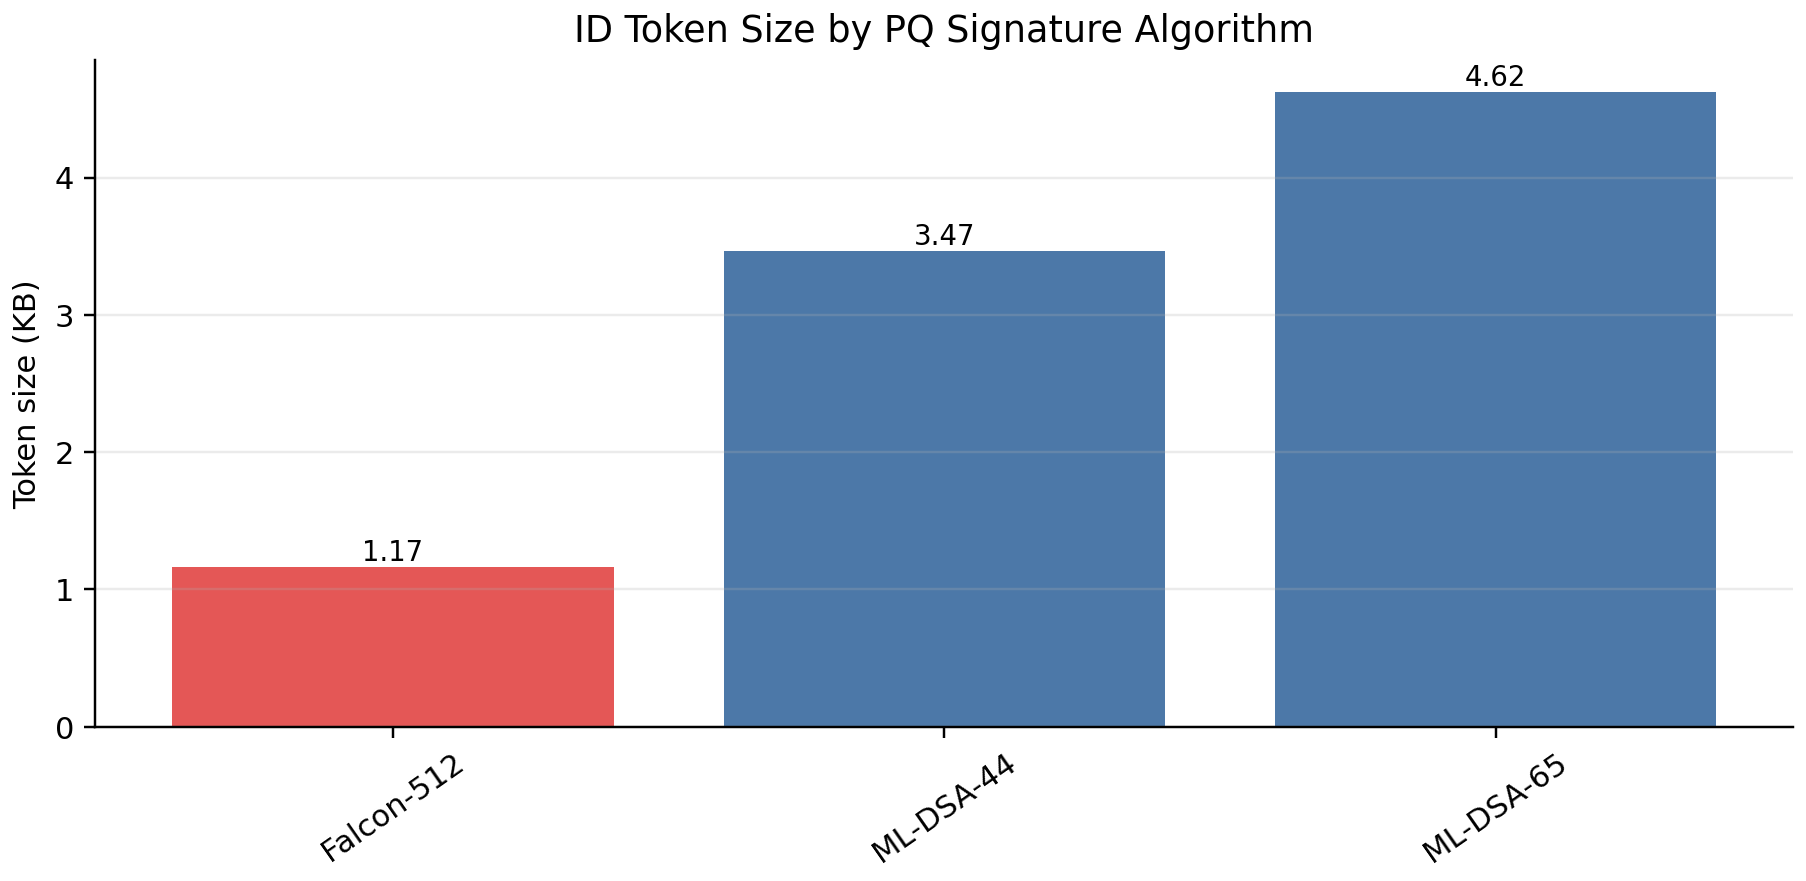
\includegraphics[width=\columnwidth]{figures/fig_token_sizes.png}
                \caption{ID token size by PQ signature algorithm (stored benchmarks).}
                \label{fig:jwt-sizes}
                \end{figure}
                \FloatBarrier
                
                \subsection{Key Tables and Protocol Summary}
                The following tables are generated from the same stored artifacts and provide the protocol-level summary rows plus JWT size/time measurements.
                \begin{table}[H]
\caption{Protocol-level benchmark summary.}
\label{tab:protocol-summary}
\centering
\setlength{\tabcolsep}{3pt}%
\renewcommand{\arraystretch}{1.05}%
\resizebox{0.98\columnwidth}{!}{%
\begin{tabular}{p{4.2cm}p{4.4cm}rrrp{1.2cm}}
\toprule\rowcolor{black!5}
Operation & Configuration & Mean (ms) & Median (ms) & Stdev (ms) & Iters \\
\midrule
End-to-End OIDC Flow & Complete Authorization Code Flow & 0.2049 & 0.1729 & 0.0859 & 20 \\
Full KEMTLS Handshake & Kyber512 + ML-DSA-44 & 0.0409 & 0.0387 & 0.0129 & 50 \\
\bottomrule
\end{tabular}}
\end{table}

                \begin{table}[H]
\caption{JWT creation performance and token sizes.}
\label{tab:jwt-sizes}
\centering
\setlength{\tabcolsep}{3pt}%
\renewcommand{\arraystretch}{1.05}%
\resizebox{0.98\columnwidth}{!}{%
\begin{tabular}{p{3.2cm}rrrp{1.2cm}r}
\toprule\rowcolor{black!5}
Algorithm & Mean (ms) & Median (ms) & Stdev (ms) & Iters & Size (B) \\
\midrule
Falcon-512 & 0.2461 & 0.2550 & 0.0277 & 100 & 1193 \\
ML-DSA-44 & 0.0812 & 0.0687 & 0.0342 & 100 & 3549 \\
ML-DSA-65 & 0.1197 & 0.1074 & 0.0605 & 100 & 4734 \\
\bottomrule
\end{tabular}}
\end{table}

                \FloatBarrier
                
                \subsection{Additional Visualizations}
                These additional visualizations use the stored mean and standard-deviation fields and highlight variability and size-vs-time tradeoffs.
                \begin{figure}[h]
                \centering
                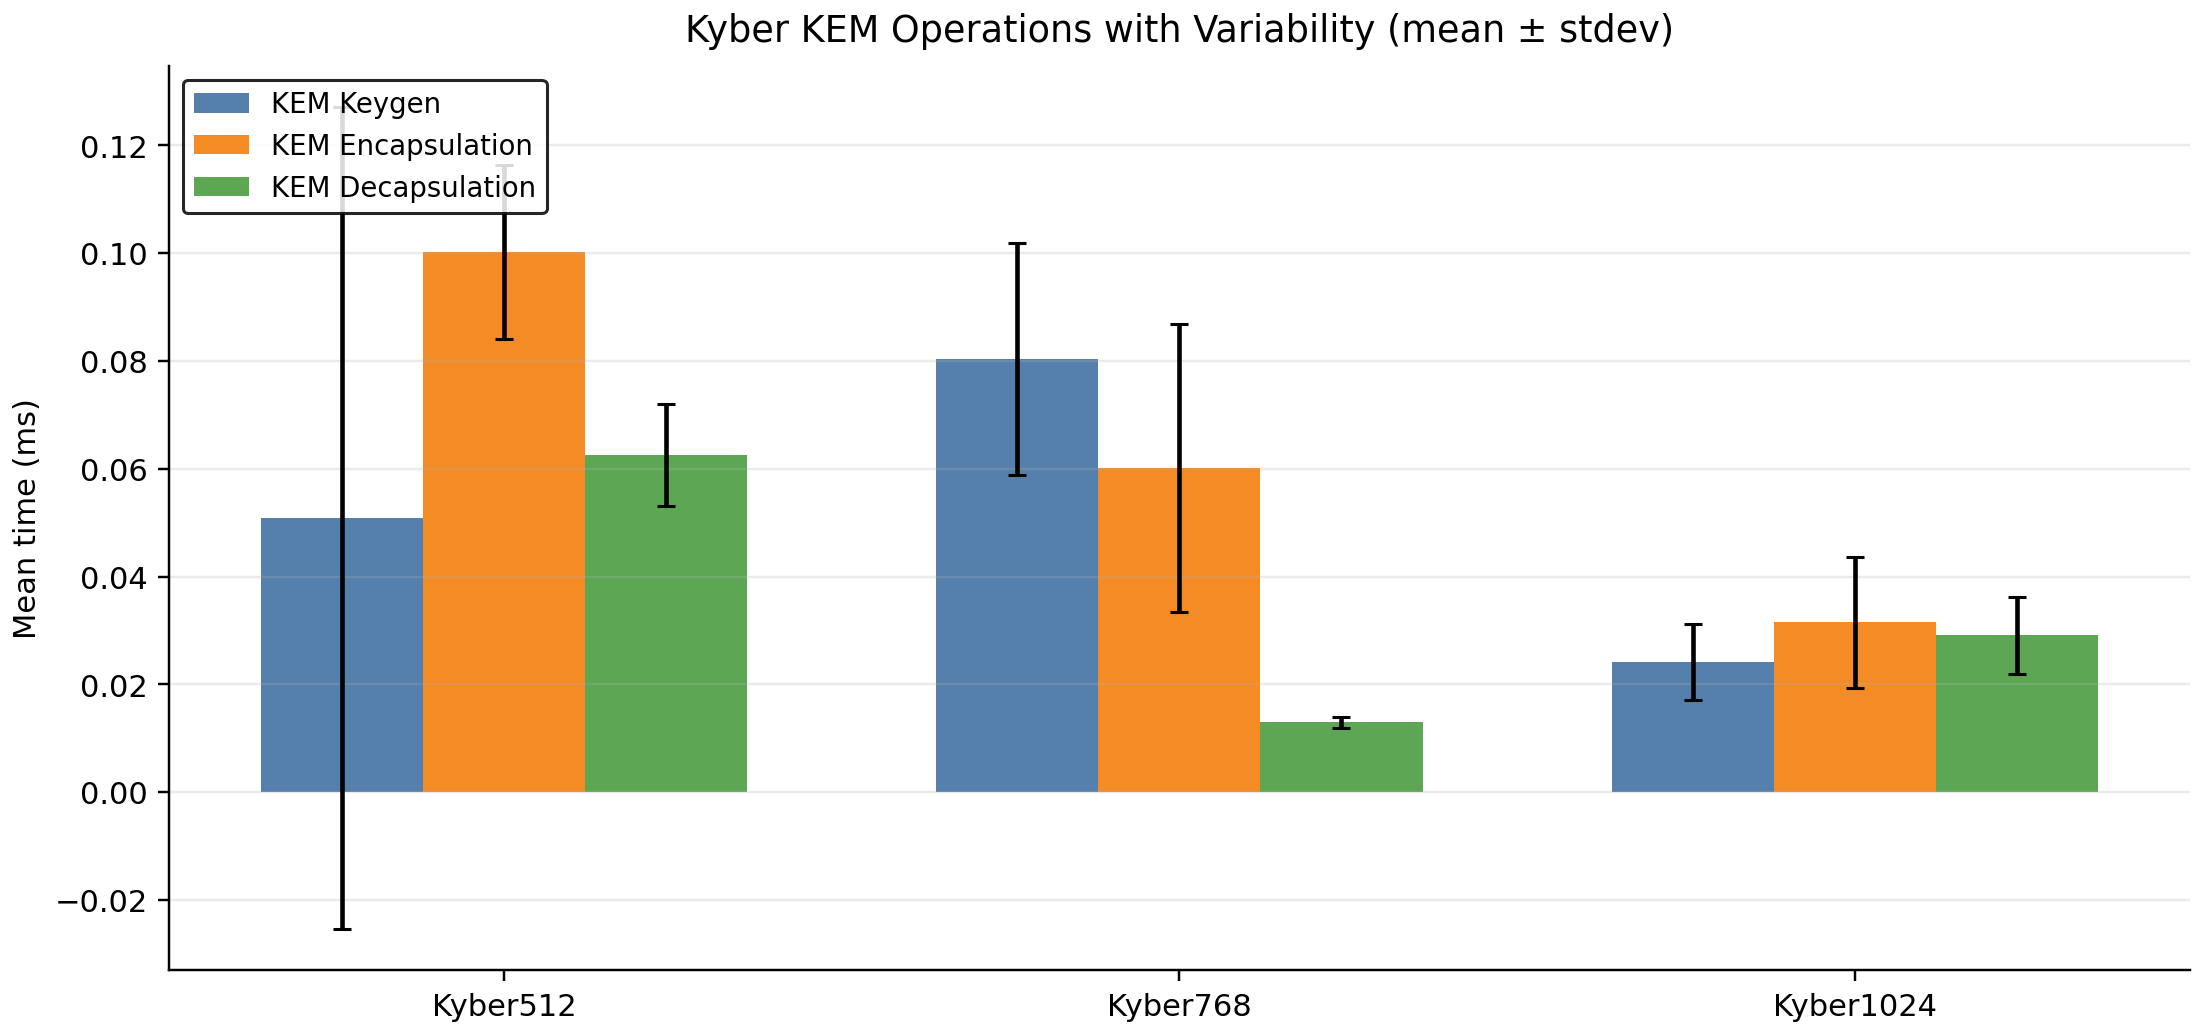
\includegraphics[width=\columnwidth]{figures/fig_kem_ops_errorbars.png}
                \caption{KEM operations with variability (mean \(\pm\) stdev), derived from stored results.}
                \label{fig:kem-errorbars}
                \end{figure}
                
                \begin{figure}[h]
                \centering
                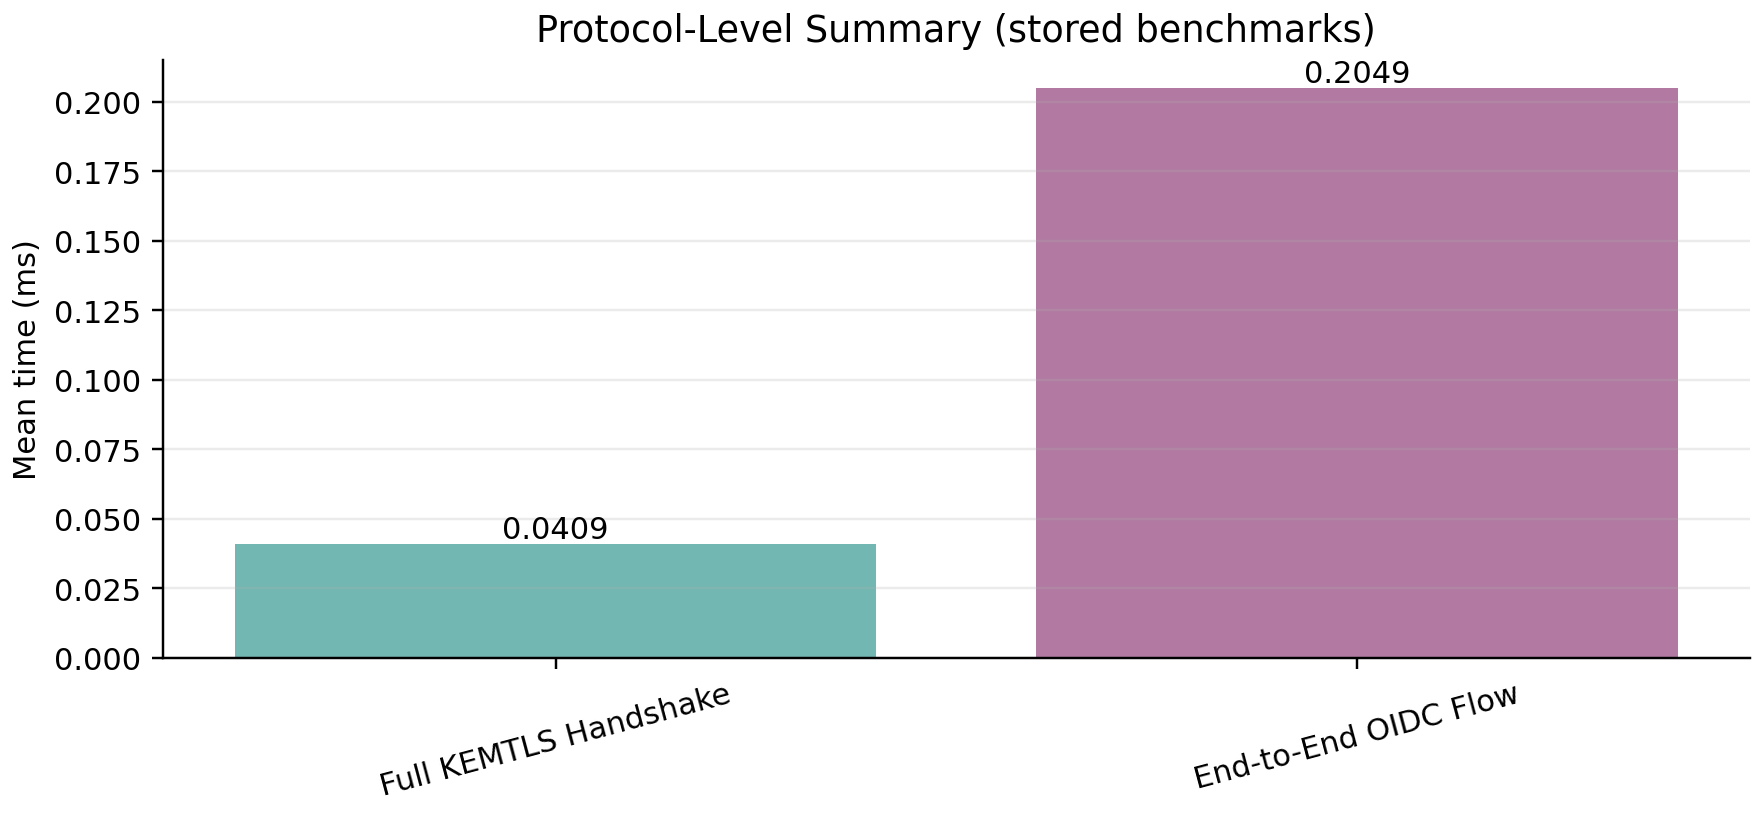
\includegraphics[width=\columnwidth]{figures/fig_protocol_summary.png}
                \caption{Protocol-level benchmark summary (mean ms), derived from stored results.}
                \label{fig:protocol-summary}
                \end{figure}
                
                \begin{figure}[h]
                \centering
                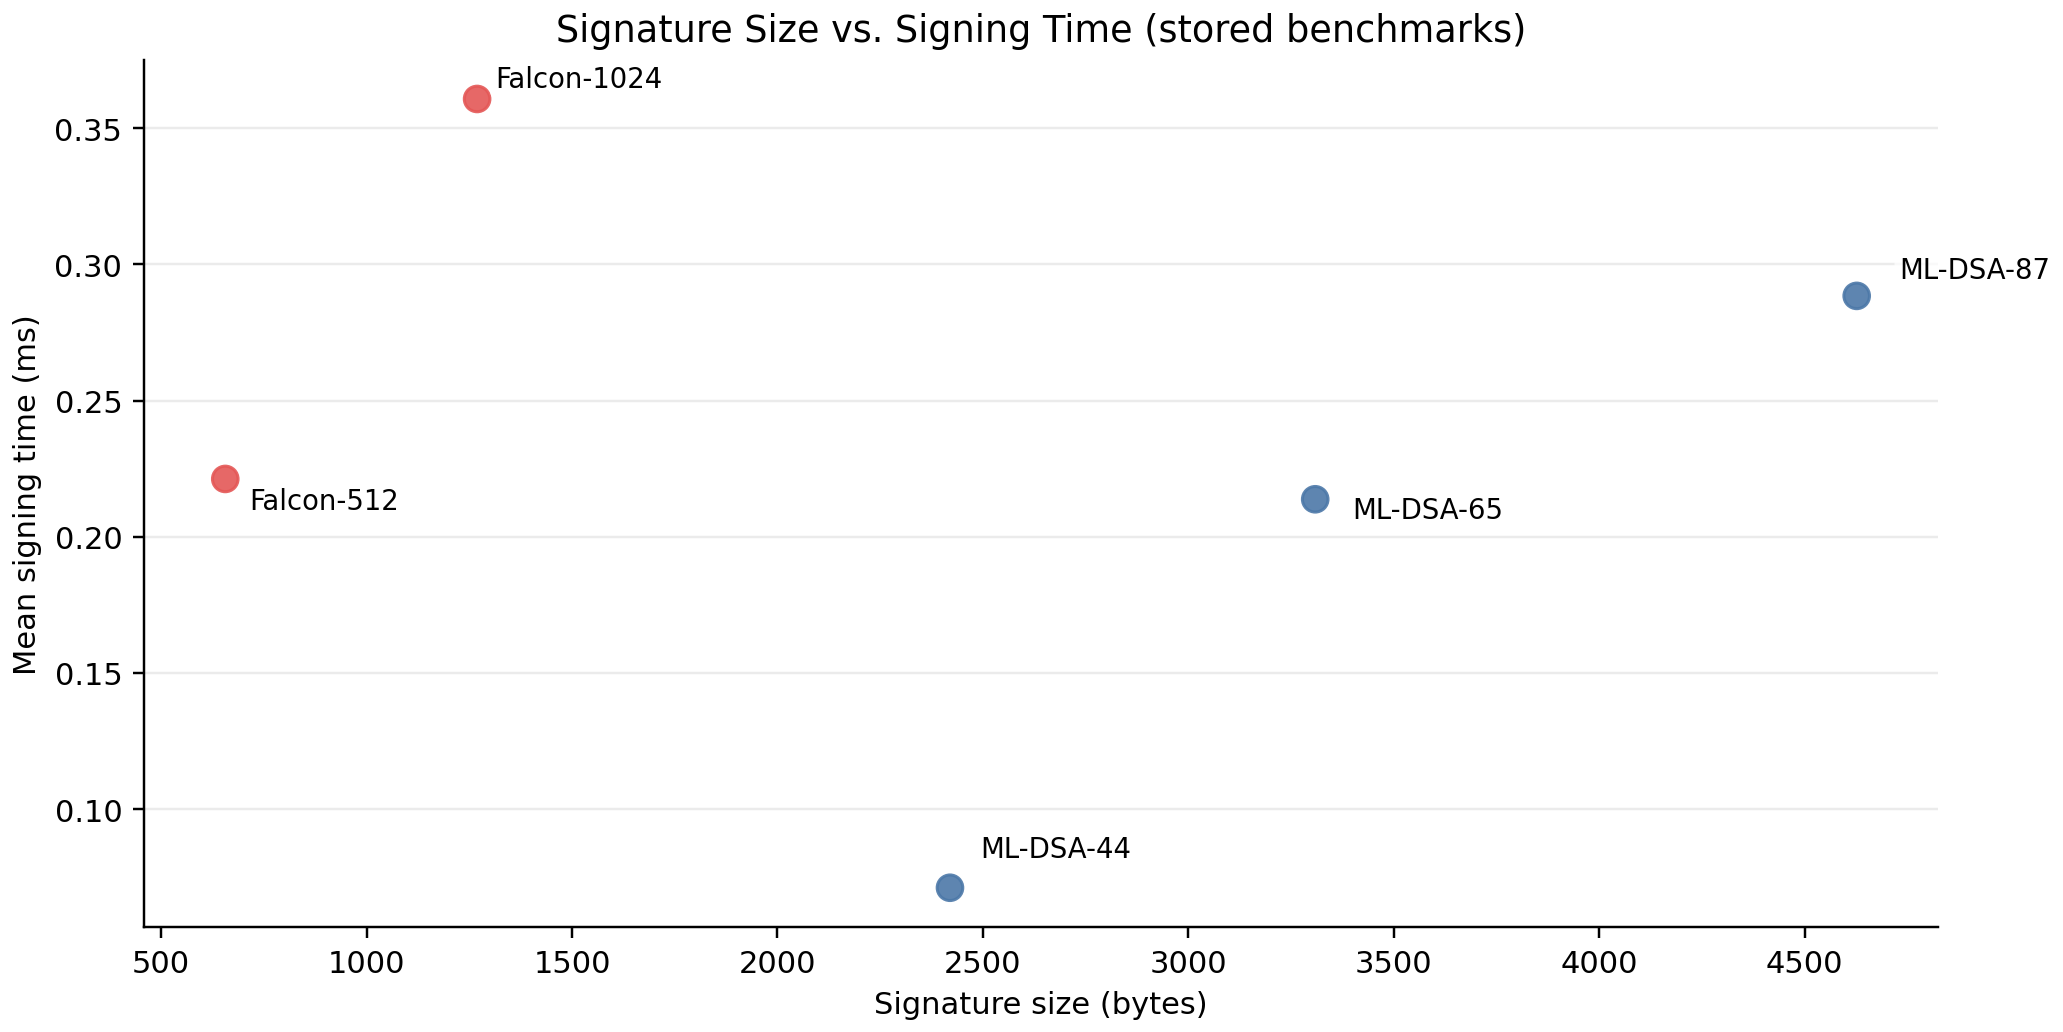
\includegraphics[width=\columnwidth]{figures/fig_signature_size_vs_time.png}
                \caption{Signature size vs. signing time (mean ms), derived from stored results.}
                \label{fig:sig-size-vs-time}
                \end{figure}
                
                \begin{figure}[h]
                \centering
                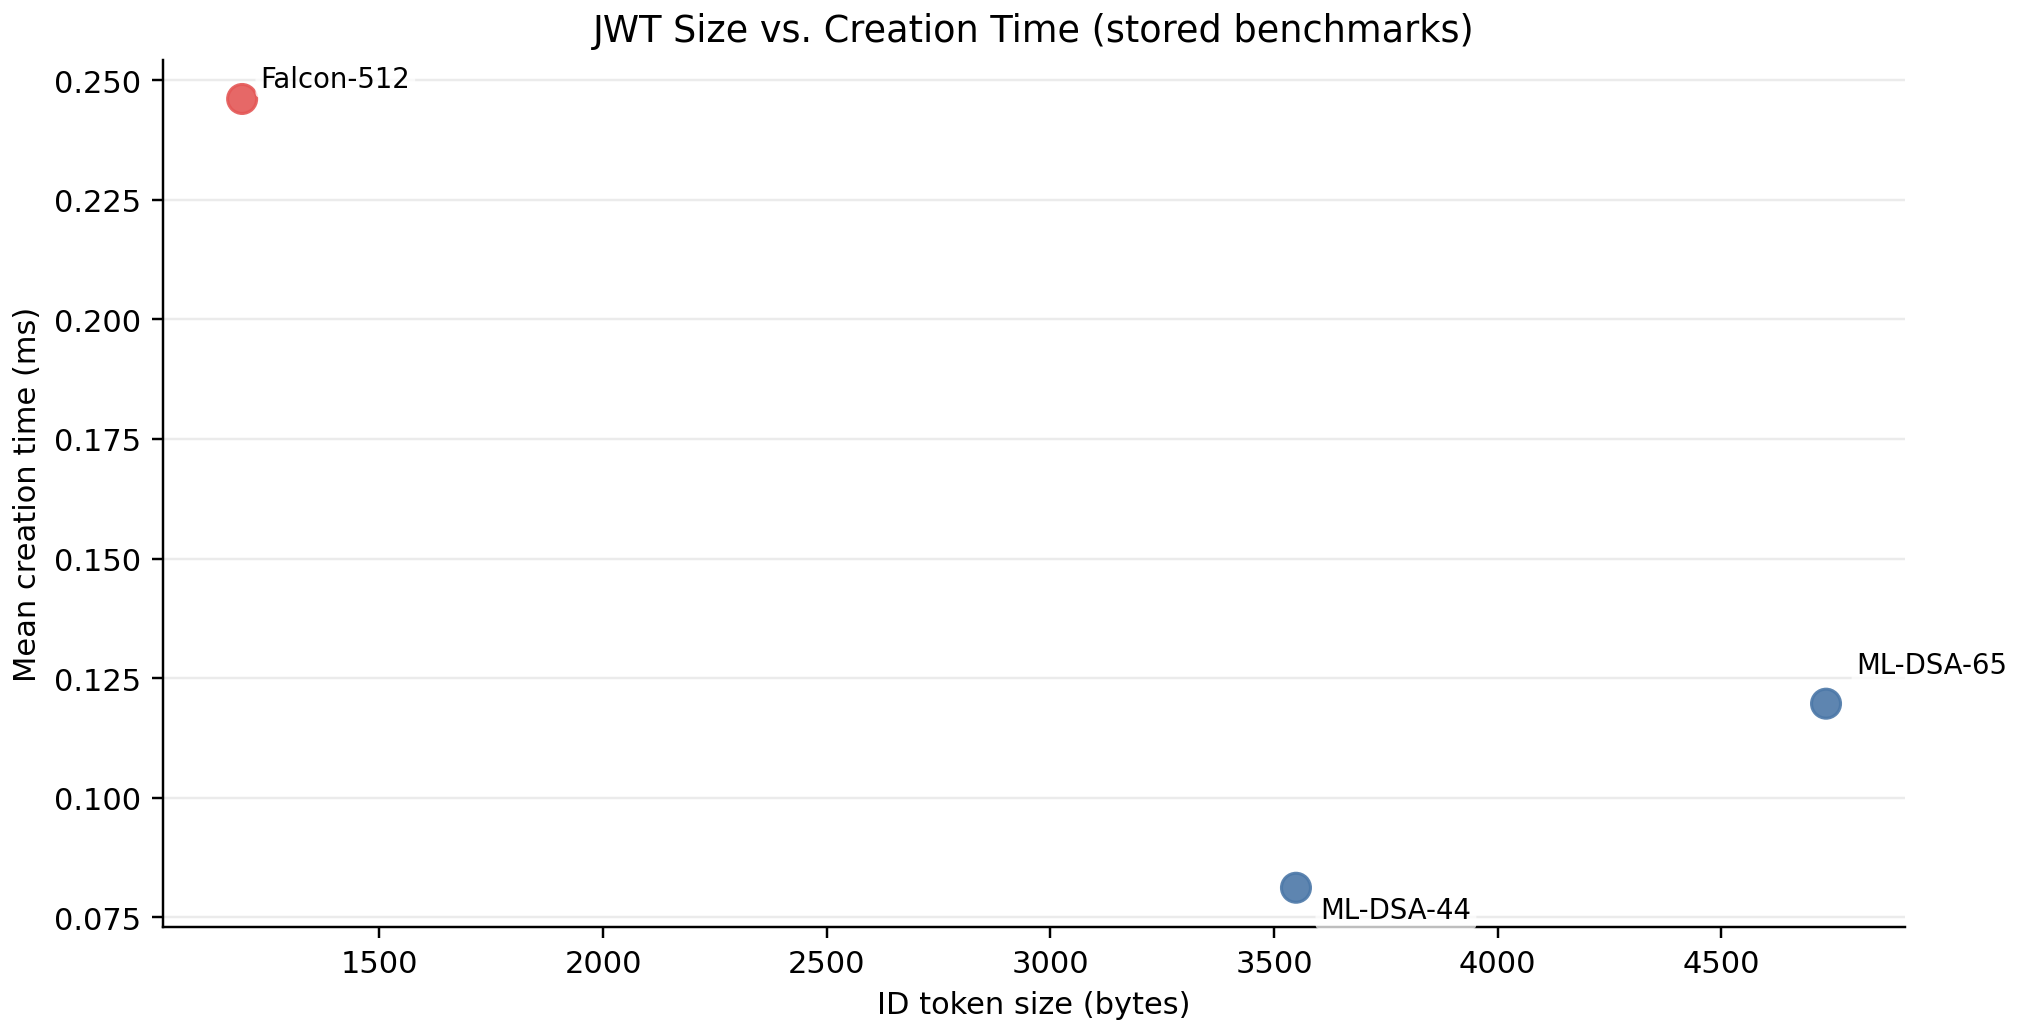
\includegraphics[width=\columnwidth]{figures/fig_jwt_size_vs_time.png}
                \caption{JWT ID token size vs. creation time (mean ms), derived from stored results.}
                \label{fig:jwt-size-vs-time}
                \end{figure}
                % Allow the next section to start on the same page if there is room.
                
                \section{Methodology}
                \subsection{Benchmark Data Provenance}
                All numeric results in this report are taken from the checked-in benchmark artifacts:
                \codepath{benchmark_results/benchmark_results.csv} and \codepath{benchmark_results/benchmark_results.json}. The plotting and tabulation code in \codepath{report/generate_assets.py} reads these inputs and produces:
                \begin{itemize}
                  \item figures under \codepath{report/figures/}, and
                  \item LaTeX table fragments under \codepath{report/tables/}.
                \end{itemize}
                \subsection{Execution Model}
                The benchmark runner (\codepath{src/benchmarks/run_benchmarks.py}) is an in-process microbenchmark suite for cryptographic operations and for prototype flows. The harness uses \texttt{time.perf\_counter()} around the measured operation and aggregates mean/median/stdev/min/max over a fixed number of iterations per operation (recorded in the corresponding artifact row).
                
                The OIDC-style flow in the repository follows the structure of OAuth~2.0 authorization code exchange~\cite{rfc6749} and uses JWT/JWS token containers~\cite{rfc7519,rfc7515}. Key expansion in the KEMTLS-style workflow is consistent with HKDF usage~\cite{rfc5869}; however, the measured protocol-level rows remain in-process benchmarks and should not be interpreted as networked TLS~1.3 latency~\cite{rfc8446}.
                
                \subsection{What ``End-to-End'' Means Here}
                The ``End-to-End OIDC Flow'' item in the stored results corresponds to a complete authorization-code style sequence executed within one Python process. It includes token issuance and ID token verification using the PQ-JWT handler. In the Flask UI (\texttt{ui/app.py}), the UserInfo step is intentionally simplified (direct user lookup) rather than a fully standards-conformant UserInfo endpoint that validates bearer access tokens.
                
                \section{Algorithms and Parameters}
                \subsection{KEM: Kyber Variants}
                The benchmark dataset includes Kyber512, Kyber768, and Kyber1024 for key generation, encapsulation, and decapsulation. These correspond to the Kyber/ML-KEM family standardized as ML-KEM in FIPS~203~\cite{fips203}. The stored artifacts also record encapsulation ciphertext sizes (bytes) for each parameter set.
                
                \subsection{Signatures: ML-DSA and Falcon}
                The dataset includes ML-DSA-44/65/87 (FIPS~204~\cite{fips204}) and Falcon-512/1024 (NIST PQC project~\cite{nist-pqc}) across key generation, signing, and verification. The stored artifacts include signature sizes (bytes) for signing operations.
                
                \subsection{JWT: PQ-Signed ID Tokens}
                JWT creation and verification are benchmarked for ML-DSA-44, ML-DSA-65, and Falcon-512. The stored artifacts include the ID token sizes (bytes) produced by the corresponding implementation.
                
                \section{Scope and Limitations}
                The implementation is a prototype and microbenchmark suite. The following scope constraints are important for interpretation:
                \begin{itemize}
                  \item \textbf{Microbenchmarks:} all timings are in-process measurements and should not be interpreted as network latency.
                  \item \textbf{KEMTLS handshake metric:} ``Full KEMTLS Handshake'' is a repository-implemented simulation (Kyber operations plus key derivation), not a socket-level handshake between \texttt{KEMTLSClient} and \texttt{KEMTLSServer}.
                  \item \textbf{UserInfo in the UI demo:} the UI uses direct user lookup for the final step; the demo UserInfo handler returns \texttt{invalid\_token} and the client-side method is not implemented.
                \end{itemize}
                \section{Development Status, Novelty, and Future Work}
                In its current form, the codebase serves as an end-to-end demonstrator for PQ-protected identity and token issuance. It integrates (i) PQ primitives, (ii) a KEMTLS-inspired key-establishment workflow~\cite{kemtls}, and (iii) an OIDC-style authorization-code flow exposed through repeatable UI and API endpoints.
                
                \subsection{What is Novel in This Repository}
                The contribution is primarily \textit{integration and reproducibility}: one codebase connects PQ KEM and signature primitives with an identity-token flow, and the report is generated from checked-in benchmark artifacts through a deterministic pipeline. This keeps the results auditable and the demonstration repeatable.
                
                \subsection{Future Scope Toward Deployment}
                To move from a demonstrator to a deployable system, the following work is needed:
                \begin{itemize}
                  \item \textbf{Standards-aligned OIDC behavior:} complete token validation for UserInfo, align endpoint behavior with OIDC Core, and add security checks (nonce/state handling, error semantics, token lifetime) consistent with OAuth/OIDC security guidance~\cite{oidc-core,rfc6749,rfc6819,rfc6750,rfc7636}.
                  \item \textbf{Networked transport integration:} connect the OIDC endpoints to a real KEMTLS-enabled transport (client/server over sockets) and measure networked latency under concurrency.
                  \item \textbf{Key management and hardening:} secure key storage, rotation, and audit logging; isolate cryptographic operations; add threat-model-driven checks.
                  \item \textbf{Operational readiness:} configuration management, CI for tests/benchmarks, and packaging/deployment patterns suitable for production environments.
                  \item \textbf{Interoperability and hybrid modes:} evaluate PQ-hybrid handshakes and token signing options for incremental deployment and compatibility.
                  \item \textbf{Security analysis and robustness:} add a clear threat model, formalize trust boundaries (UI/server/crypto), and perform negative testing and fuzzing for token parsing and protocol state.
                \end{itemize}
                \subsection{Roadmap Direction (Brief)}
                A practical sequence of next steps toward a stronger research artifact and, later, a deployment-oriented implementation is:
                \begin{itemize}
                  \item \textbf{Near-term (weeks):} tighten protocol semantics and error handling against OAuth/OIDC requirements~\cite{rfc6749,oidc-core}; implement bearer-token validation for UserInfo~\cite{rfc6750}; add PKCE support for the authorization-code flow~\cite{rfc7636}; expand negative tests.
                  \item \textbf{Mid-term (1--2 months):} integrate a networked client/server transport for the KEMTLS-inspired layer; measure latency under concurrency; add key storage and rotation interfaces; document an explicit threat model with testable assumptions~\cite{rfc6819}.
                  \item \textbf{Long-term (semester scale):} evaluate hybrid deployment options (classical+PQ), interoperability constraints, and cross-implementation portability; extend benchmarks to include network effects and larger payloads; pursue formal validation of token parsing and state machines.
                \end{itemize}
                \section{Conclusion}
                This prototype validates the structural integration of post-quantum cryptography within established authentication protocols. The implementation maps post-quantum primitives to a KEMTLS key-establishment simulation, mitigating the latency penalties associated with massive digital signatures. The resulting transport layer supports an operational OIDC authorization flow reliant on PQ-signed JSON Web Tokens.
                
                Methodological reproducibility is enforced across the evaluation pipeline:
                \begin{itemize}
                  \item \textbf{Deterministic Evaluation:} All visual and numeric artifacts are programmatically derived from static, checked-in benchmarking datasets (CSV/JSON).
                  \item \textbf{Structural Mapping:} Abstract protocol layers are explicitly coupled to distinct codebase modules (primitives, KEMTLS, and PQ-JWT) for audibility.
                  \item \textbf{Empirical Scope:} The benchmarking suite tracks 32 execution and size metrics, isolating the isolated cryptographic overhead of the KEMTLS handshake and the integrated OIDC sequence.
                \end{itemize}
                Future efforts must transition the system from an in-process demonstrator to a networked implementation. Critical next steps involve deploying a fully compliant UserInfo endpoint, establishing a socket-bound KEMTLS transport layer, and evaluating throughput constraints under realistic network concurrency.
                
                \bibliographystyle{IEEEtran}
                \bibliography{references}
                
                \appendices
                \onecolumn
                \section{Complete Benchmark Dataset}
                \label{app:full-table}
                \begingroup
                \small
                \setlength{\LTleft}{0pt}
                \setlength{\LTright}{0pt}
                \begin{longtable}{p{2.8cm}p{2.6cm}rrrrrrr}
\caption{Complete benchmark dataset (derived from stored benchmark artifacts).} \label{tab:full-results} \\
\toprule\rowcolor{black!5}
Operation & Algorithm & Mean (ms) & Median (ms) & Stdev (ms) & Min (ms) & Max (ms) & Iters & Size (B) \\
\midrule
\endfirsthead
\caption[]{Complete benchmark dataset (derived from stored benchmark artifacts).} \\
\toprule\rowcolor{black!5}
Operation & Algorithm & Mean (ms) & Median (ms) & Stdev (ms) & Min (ms) & Max (ms) & Iters & Size (B) \\
\midrule
\endhead
\midrule
\multicolumn{9}{r}{Continued on next page} \\
\midrule
\endfoot
\bottomrule
\endlastfoot
End-to-End OIDC Flow & Complete Authorization Code Flow & 0.2049 & 0.1729 & 0.0859 & 0.1399 & 0.4612 & 20 & 0 \\
Full KEMTLS Handshake & Kyber512 + ML-DSA-44 & 0.0409 & 0.0387 & 0.0129 & 0.0381 & 0.1296 & 50 & 0 \\
JWT Creation & Falcon-512 & 0.2461 & 0.2550 & 0.0277 & 0.1854 & 0.3207 & 100 & 1193 \\
JWT Creation & ML-DSA-44 & 0.0812 & 0.0687 & 0.0342 & 0.0465 & 0.1939 & 100 & 3549 \\
JWT Creation & ML-DSA-65 & 0.1197 & 0.1074 & 0.0605 & 0.0649 & 0.3922 & 100 & 4734 \\
JWT Verification & Falcon-512 & 0.0557 & 0.0468 & 0.0167 & 0.0457 & 0.1767 & 100 & 0 \\
JWT Verification & ML-DSA-44 & 0.0435 & 0.0426 & 0.0064 & 0.0417 & 0.1051 & 100 & 0 \\
JWT Verification & ML-DSA-65 & 0.0607 & 0.0597 & 0.0041 & 0.0587 & 0.0904 & 100 & 0 \\
KEM Decapsulation & Kyber1024 & 0.0291 & 0.0269 & 0.0071 & 0.0207 & 0.0460 & 100 & 0 \\
KEM Decapsulation & Kyber512 & 0.0625 & 0.0592 & 0.0095 & 0.0577 & 0.1456 & 100 & 0 \\
KEM Decapsulation & Kyber768 & 0.0129 & 0.0127 & 0.0010 & 0.0125 & 0.0199 & 100 & 0 \\
KEM Encapsulation & Kyber1024 & 0.0315 & 0.0240 & 0.0122 & 0.0228 & 0.0663 & 100 & 1568 \\
KEM Encapsulation & Kyber512 & 0.1003 & 0.0994 & 0.0161 & 0.0763 & 0.2290 & 100 & 768 \\
KEM Encapsulation & Kyber768 & 0.0601 & 0.0736 & 0.0267 & 0.0248 & 0.1289 & 100 & 1088 \\
KEM Keygen & Kyber1024 & 0.0241 & 0.0220 & 0.0070 & 0.0182 & 0.0587 & 100 & 0 \\
KEM Keygen & Kyber512 & 0.0508 & 0.0494 & 0.0763 & 0.0162 & 0.7798 & 100 & 0 \\
KEM Keygen & Kyber768 & 0.0804 & 0.0765 & 0.0216 & 0.0707 & 0.2817 & 100 & 0 \\
Sign & Falcon-1024 & 0.3607 & 0.3561 & 0.0161 & 0.3466 & 0.4443 & 100 & 1269 \\
Sign & Falcon-512 & 0.2212 & 0.2399 & 0.0318 & 0.1772 & 0.2858 & 100 & 656 \\
Sign & ML-DSA-44 & 0.0711 & 0.0571 & 0.0362 & 0.0354 & 0.1982 & 100 & 2420 \\
Sign & ML-DSA-65 & 0.2138 & 0.1730 & 0.1301 & 0.0523 & 0.6883 & 100 & 3309 \\
Sign & ML-DSA-87 & 0.2884 & 0.2275 & 0.1641 & 0.0791 & 0.7371 & 100 & 4627 \\
Signature Keygen & Falcon-1024 & 15.8008 & 14.5125 & 3.5410 & 12.7385 & 28.5174 & 100 & 0 \\
Signature Keygen & Falcon-512 & 5.3442 & 4.8952 & 1.5479 & 3.9154 & 12.6677 & 100 & 0 \\
Signature Keygen & ML-DSA-44 & 0.0325 & 0.0284 & 0.0209 & 0.0273 & 0.2341 & 100 & 0 \\
Signature Keygen & ML-DSA-65 & 0.0500 & 0.0424 & 0.0133 & 0.0418 & 0.1249 & 100 & 0 \\
Signature Keygen & ML-DSA-87 & 0.0683 & 0.0655 & 0.0118 & 0.0643 & 0.1769 & 100 & 0 \\
Verify & Falcon-1024 & 0.0655 & 0.0640 & 0.0060 & 0.0632 & 0.1167 & 100 & 0 \\
Verify & Falcon-512 & 0.0440 & 0.0499 & 0.0112 & 0.0336 & 0.1121 & 100 & 0 \\
Verify & ML-DSA-44 & 0.0262 & 0.0256 & 0.0028 & 0.0251 & 0.0524 & 100 & 0 \\
Verify & ML-DSA-65 & 0.0431 & 0.0418 & 0.0035 & 0.0405 & 0.0572 & 100 & 0 \\
Verify & ML-DSA-87 & 0.0893 & 0.0648 & 0.0454 & 0.0629 & 0.1870 & 100 & 0 \\
\end{longtable}

                \endgroup
                
                \section{Raw CSV Snapshot (for audit)}
                \begingroup
                \small
                \lstinputlisting[caption={benchmark\_results.csv (snapshot copy packaged with this report)}]{data/benchmark_results.csv}
                \endgroup

                \section{Public Repository for Supplementary Materials}
                A public Google Drive folder is provided to support peer review and reproducibility. It contains:
                \begin{itemize}
                    \item Detailed project documentation
                    \item Demonstration video of the system
                    \item Benchmark results in .json, .xls, and .pdf formats
                    \item Generated graphs and performance analysis plots
                    \item Additional artifacts and supporting information
                \end{itemize}
                Available at: \url{https://drive.google.com/drive/folders/10vI3nyteF3sNEIiO031Q8r9rMdjAiOOY}
                
                \end{document}
                